\externaldocument{modelling}

\section{Experiments and Results}
For all the plots of the experiments the red curve indicates the tumour cell density, the blue curve the ECM density and the green curve the MDE concentration. In all of the experiments we used the value of $\epsilon = 0.01$ to match the inital conditions from \cite{anderson_mathematical_2000} and \cite{Kolev2010}. \newline 


\subsection{Two dimensional Results without Proliferation}
\subsubsection{Replicating results}
We will start with replicating the experiment from  Anderson et al.\cite{anderson_mathematical_2000}, Figure~\ref{fig:unadjsuted_replication}, trying to make our curves fit the results of their experiment. 

%naming convention of figures: d0_d1_d2_eta_alpha_beta_gamma_mu1_mu2

\begin{figure}[h]
    \centering
    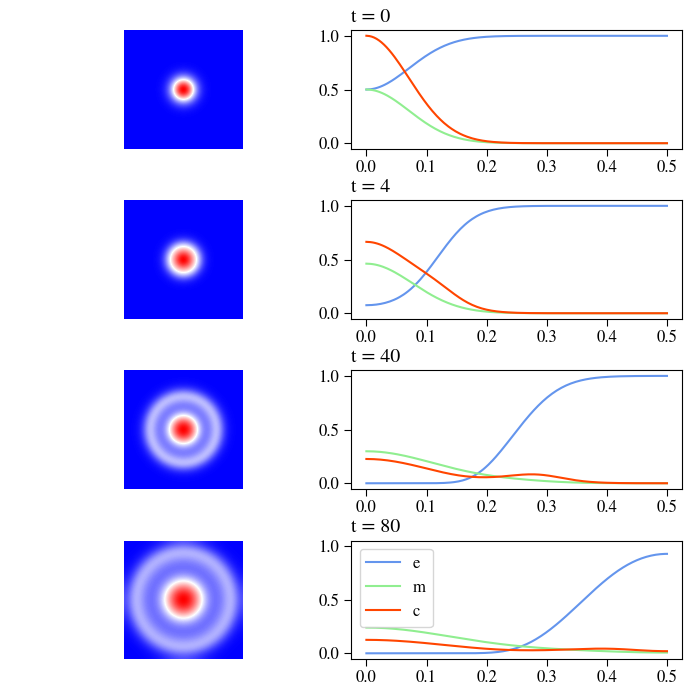
\includegraphics[width=0.7\textwidth]{resources/images/first_replication_results.png}
    \caption{Images on left side 2D tumour cell density plots of the experiment, images on right side results produced by applying Plot Over Line tool}
    \label{fig:unadjsuted_replication}
\end{figure}

We start with the same parameters as in Anderson et al's first $1D$ experiment: $d_c = 0.001, d_m = 0.001, \gamma = 0.005, \eta = 10, \alpha = 0.1, \beta = 0, \mu_1 = 0, \mu_2 = 0$. Figure~\ref{fig:unadjsuted_replication} shows these results for four different points in time. Since our experiments are preformed in two dimensions you can see on the left side the two dimensional plots of the tumour cell density and on the right side you can see plots produced by applying the Plot Over Line tool confiugrated like described in the section~\ref{sec:method}, where there is not only the tumour cell density visible but also the matrix degrading enzymes concentration and the extracellular matrix concentration. We choose these points in time, because we used a different timescale than Anderson et al. and as you will later see, our time points capture the effects that can be observed studying their results quite well, which implies that for every time step Anderson et al. did we had to do 4. The problem with the two dimensional plots is that as you can see overlaying the different variables of tumour cell density, MDE concentration and ECM concentration, makes the plots unreadable, so you can only show one at a time, additionally to this it is harder to estimate values for $c$, $e$ and $m$ at different locations in space and time. These problems are solved using the Plot Over Line tool, as you can see in the plots of figure~\ref{fig:unadjsuted_replication} on the right side the curves for the three variables are clearly distinguishable and we can estimate their values spacially and temporarily better. This is why for most experiments we resort to using only the results produced by the Plot Over Line method instead of full 2D simulation images, this makes evaluating and comparing the respective experiments a lot easier and still captures all occuring effects. \newline
Starting from the inital values at $t=0$ we see that after four time steps a very small secession is starting to form for the tumour cell density at $x\approx 0.1$. Diffusion and Haptotaxis have stretched the curve for the tumour cells along the x-axis as did diffusion for the MDEs. The ECM has  been visibly degraded at the origin, being still fully present in outer regions exceeding $x\approx 0.2$.\newline
The next image shows the simulation after 40 timesteps; we see that the secession of the tumour cell concentration of the previous point in time has been propagated to form a small hill at the leading edge of the tumour cells invading the surrounding tissue, this effect is due to the haptotatic influence, which pulls the tumour cells further into the accessible area towards higher values of $\nabla (c \nabla e)$, creating a seperation for the tumour cells, where the other part is still oriented towards the origin. The MDEs also continue their diffusion into the area, degrading the ECM in their wake.\newline 
In the last image, after 80 simulation time steps, we see that as well the hill that has formed at the leading edge of the tumour cells as well as the concentration of tumour cells at the origin, have flattened visibly and striving to take on a constant concentration throughout space, though we can still clearly distinguish both areas. If we were to look at the simulation at later points in time, the curve will flatten even more, since with more time the ECM will be further degraded and therefore the haptotactic flux coefficient $\gamma$ will lose its significance, leaving the movement of the tumour cells to diffusion only and spreading them constantly along the x-axis. The curve for the MDEs will also flattened due to diffusion,with the MDEs degrading the rest of the extracellular matrix molecules decrease their concentration further and the MDE concentration will increase over time due to no limiting factors in this experiment and on-going production contributed by the tumour cells $c$.\newline
Comparing \ref{fig:unadjsuted_replication} to figure 1 in \cite{anderson_mathematical_2000}, we can see major differences. The first image showing $t=0$ looks the same, which confirms that both experiments start with the same initial values condition. In the images showing the simulation at the second time checkpoint we see that though the tumour concentration and ECM density values are approximately the same, the MDE concentration is slightly lower in our experiment, which will get more pregnant in the later images. The unevenness having formed at the leading edge of the tumour cell concentration is also slightly smaller. The differences in the third image are more striking, both $c$ and $m$ have considerably lower concentrations, yet the ECM value looks is very similar. \newline 
In our case the diffusion and haptotatic pull of the tumour cells has shown to be too stong making the invasion process into the tissue happen too fast. The last time checkpoints strengthens our findings, showing the same behaviour with ECM being approximately the same, tumour cell density and MDE concentration being clearly lower in our experiment and invasion of tissue happening too fast, leaving the lump at the origin $x=0$ too small. \newline 
This first of all confirms the initial supposition that with changing the dimension for the simulations the results also vary. We will now adjust the parameters iteratively to make the results using two dimensions mimick the results from Anderson et. al as closely as possible. For this we will start with varying the MDE production coefficient $\alpha$, to get higher concentration values for the MDEs, and change the diffusion as well as haptotaxis coefficients of the tumour cells $d_c$ and  $\gamma$, to adjust the motitlity of the tumour cells and therefore also influence the invasion speed of them into the surrouding tissue.

\begin{figure}[h]
    \centering
    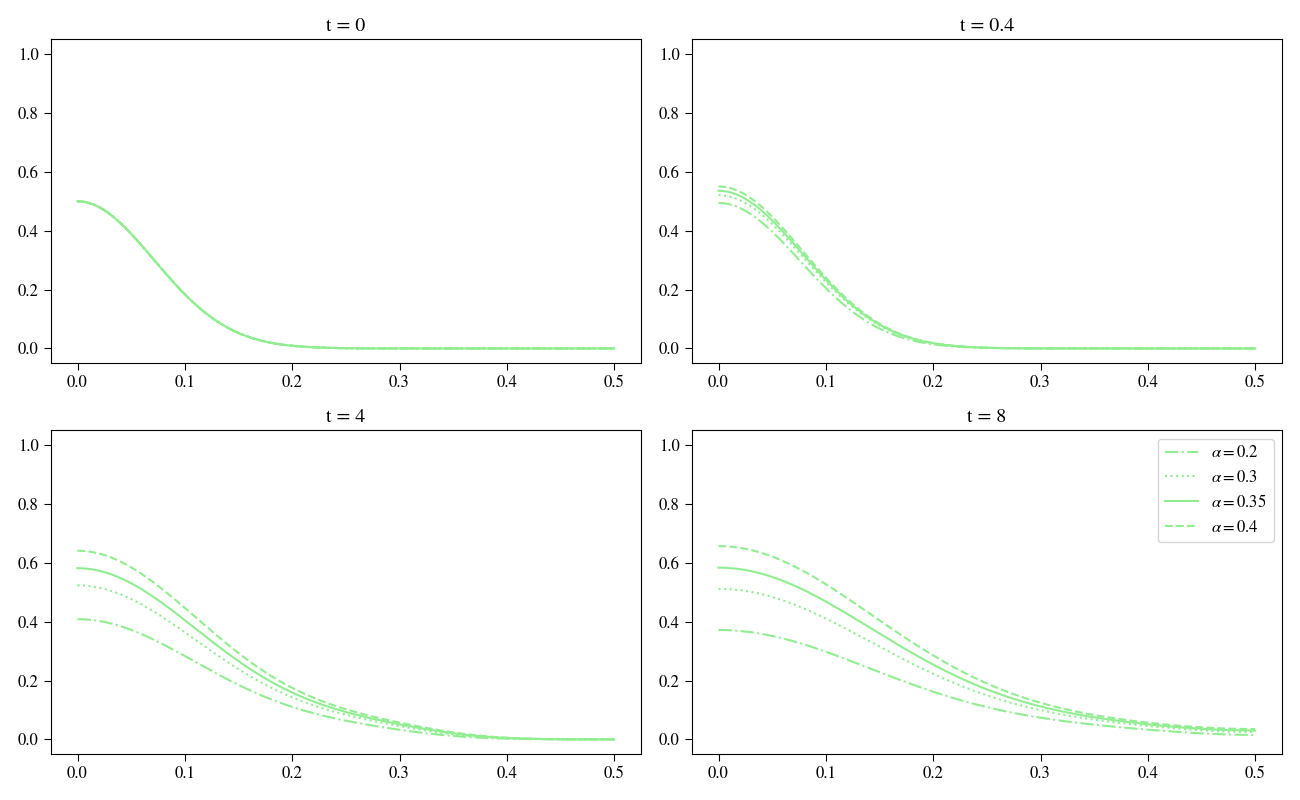
\includegraphics[width=0.8\textwidth]{resources/images/alpha_comparison.png}
    \caption{Caption}
    \label{fig:replication_alpha_comparison}
\end{figure}

\begin{figure}[h]
    \centering
    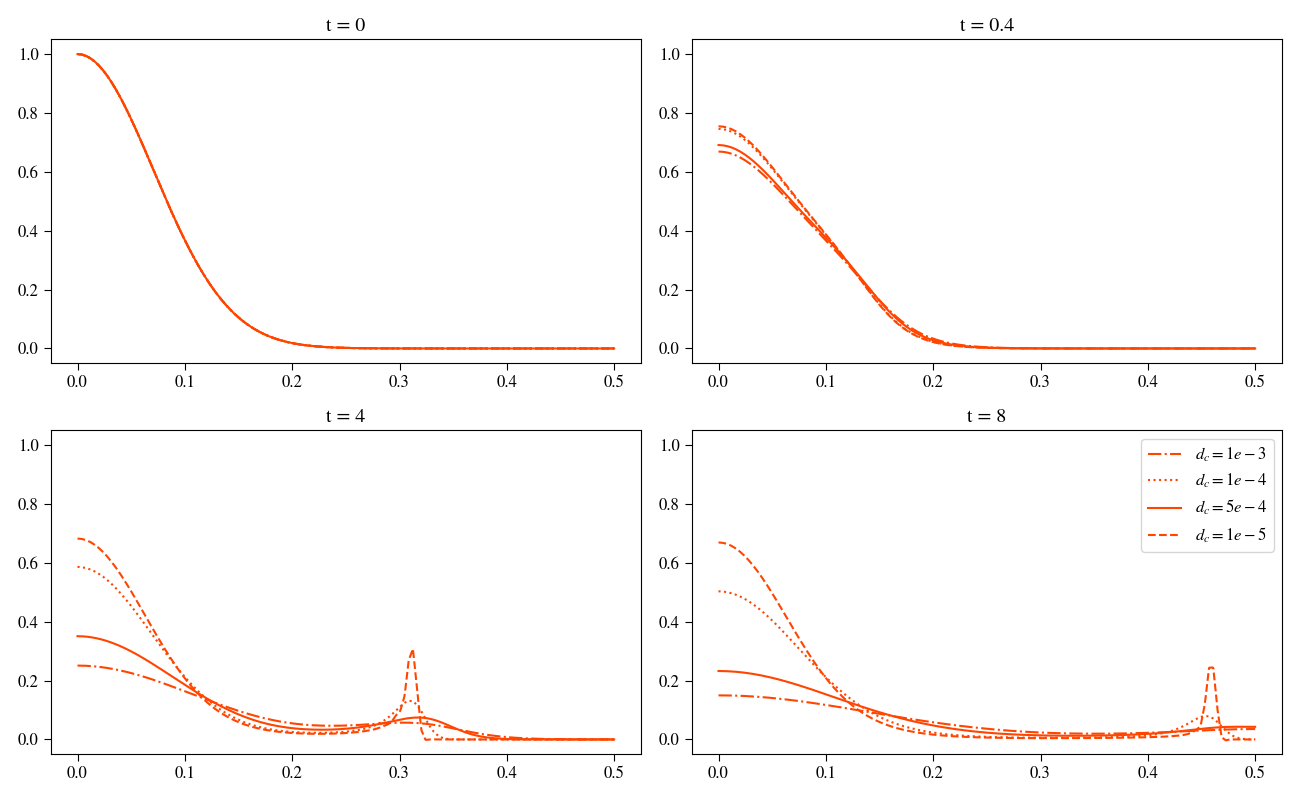
\includegraphics[width=0.8\textwidth]{resources/images/dc_comparison.png}
    \caption{Caption}
    \label{fig:replication_dc_comparison}
\end{figure}

\begin{figure}[h]
    \centering
    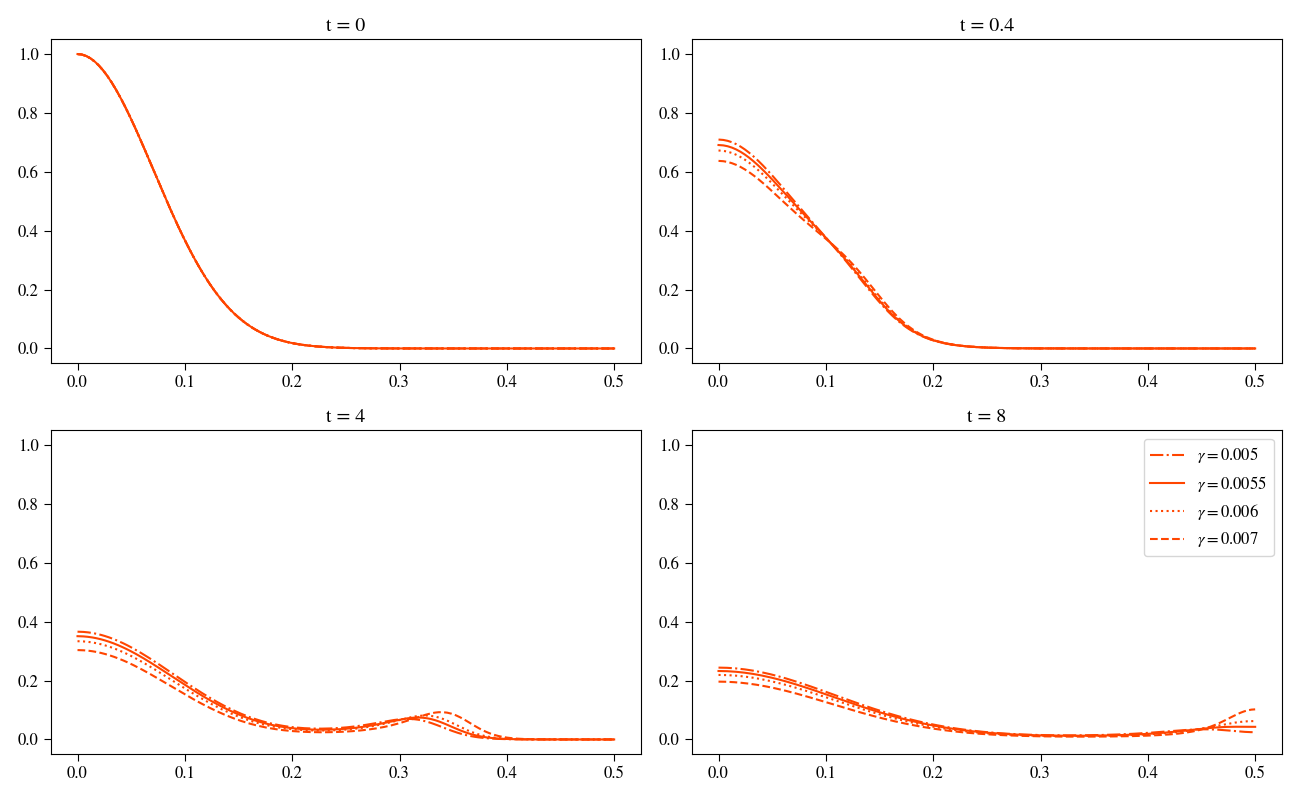
\includegraphics[width=0.8\textwidth]{resources/images/gamma_comparison.png}
    \caption{Caption}
    \label{fig:replication_gamma_comparison}
\end{figure}



Figures~\ref{fig:replication_alpha_comparison}, ~\ref{fig:replication_dc_comparison} and ~\ref{fig:replication_gamma_comparison} show these comparisons of the parameters $\alpha$, $d_c$ and $\gamma$. Comparing different values for $\alpha$ and their effect on the curve of the MDE concentration, shows in figure~\ref{fig:replication_alpha_comparison} that, especially looking at the later points in time $t=40$ and $t=80$, with values for $\alpha$ between $0.3$ and $0.4$ we will get a good approximation. The values of the original paper for the MDEs are for $t=4$ approximately $0.6$ at $x=0$ and for $t=8$ about $0.7$ at the same point in space. Fine tuning this parameter led us use $\alpha=0.35645$.\newline 
Looking at $d_c$ we chose a value of $d_c=5e-4$. Using values below $1e-5$ will result in numerical instabilities and results that are not longer useable. For $\gamma$ we made a slight adjustment upwards to $\gamma=0.0055$ to have a little bit more pull on the tumour cells outward, to match the invasion speed observed in the original paper. 
\begin{figure}[h]
    \centering
    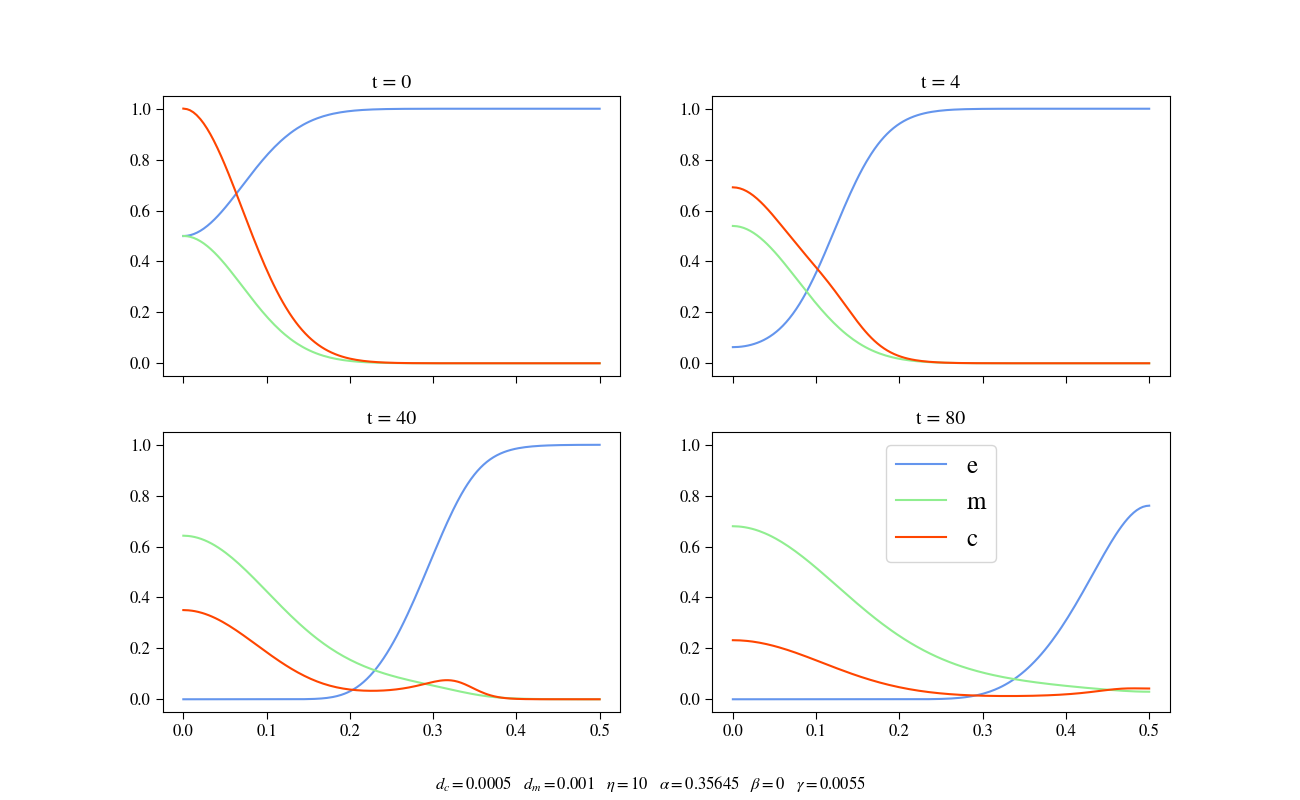
\includegraphics[width=\textwidth]{resources/images/basecase_without_proliferation.png}
    \label{fig:basecase_without_proliferation}
\end{figure}

These adjustments leave us with the final configuration for replicating the system with the curves in figure~\ref{fig:basecase_without_proliferation} and the parameter settings also seen in the same figure. Comparing our final version with the original experiment we are trying to replicate we can see that in the second point in time, at $t=4$ in our case, the values of the three curves at the $x=0$ are nearly the same, and moving farther out along the x-axis the curves mimick each other quite well. In the original experiment the bump in the curve for the tumour concentration looks more pregnant, but this is due to the differing dimensions and the rescaling of the x-axis done in Anderson et al's experiment. The two later points in time confirm the similarity with having also nealy the same values for the three curves over the whole space domain.



\subsubsection{Parameter Analysis}

Mathematical Intuition of the three curves and how the parameters interact.\newline 
From the replicated results shown in figures~\ref{fig:basecase_without_proliferation}, we saw that if we vary certain parameters one at a time the results also vary strongly. Therefore we are now going to have a look at how changing one parameter affects the output of the whole system. For this we assume the parameter values of the replicated results to be our set of baseline parameters, from there in each experiment only one parameter is changed at first, later we will also perform cross variations, where more than one parameter is changed at a time, to see how they interact and change the results. 

\subsubsection*{$d_c$ Variation}
The parameter analysed in this section describes the diffusion of the tumour cells and is integrated into the equations as being dependent on the laplacian of the tumour cells $\Delta c = (\frac{\partial^2 c}{\partial x^2} + \frac{\partial^2 c}{\partial y^2} + \frac{\partial^2 c}{\partial z^2})$. Leaving out the proliferation term our equation for $\frac{\partial c}{\partial t}$ also depends on $\gamma$ a coefficient for the haptotatic flux. The mathematical intuition is that if we will decrease $d_c$ we will see the effects of $\gamma$ taking over the simulation results for the $c$ curve, meaning that the tumour cells are more likely to drift outward and let themselves be pulled by the ECM concentration $e$, due to haptotaxis, leaving ony a little concentration at the center $x=0$, creating a bigger hill on the leading edge of the tumour concentration (below where $c \nabla e$ will be highest). On the other hand if we increase $d_c$ the effects of haptotaxis will diminish, the tumour cells will be subject to bigger diffusion pulling them more evenly into the tissue, there will be less of a leading hill being pulled outwards, since the diffusion will happen too fast, making this effect irrelevant. 
\begin{figure}[h]
    \centering
    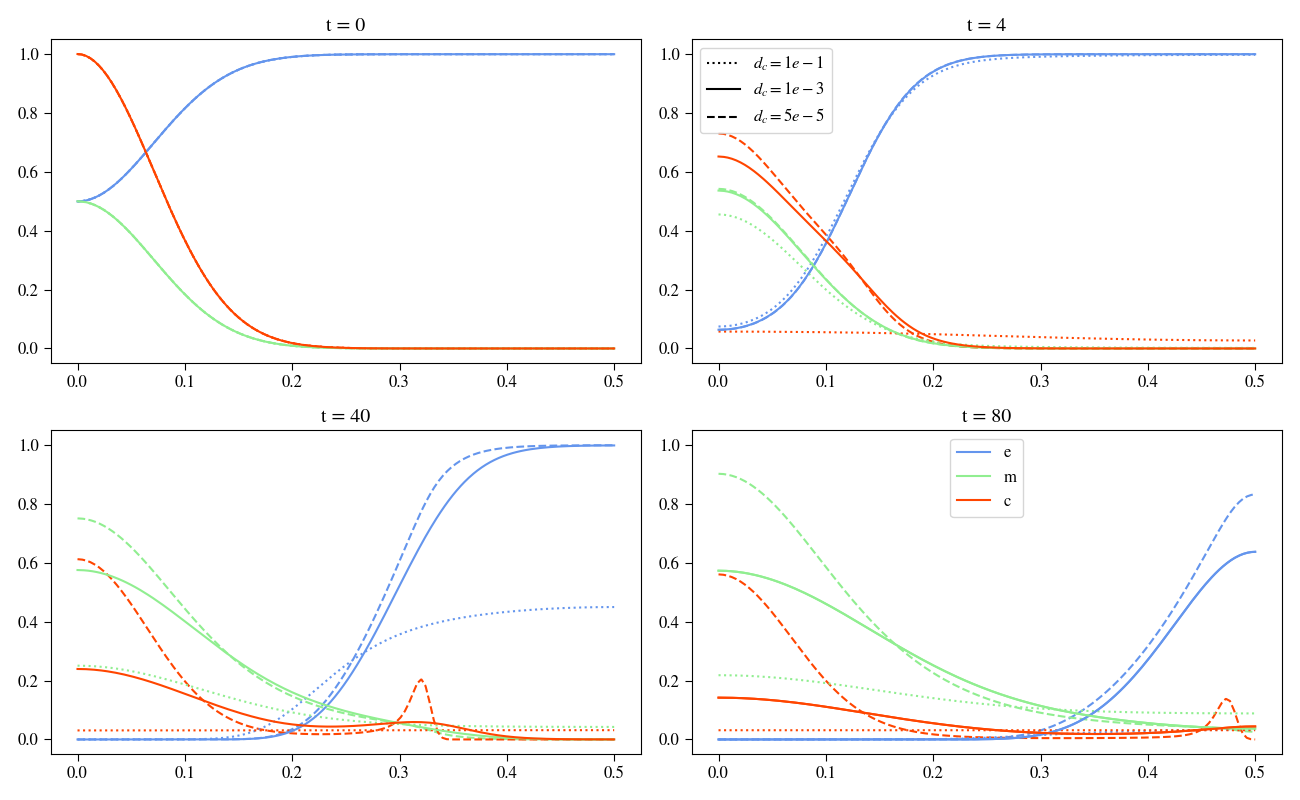
\includegraphics[width=\textwidth]{resources/images/dc_variation.png}
    \caption{Plots show results for varying $d_c$ whilst keeping the other parameters constant, in the images you can see the effects of $d_c=5e-5$ in the dashed curve, $d_c=1e-1$ in the dotted curve and $d_c=5e-4$ in the solid line.}
    \label{fig:dc_comparison}
\end{figure}
Looking at both experiments in figure~\ref{fig:dc_comparison}, we can see these assumptions confirmed. The smaller $d_c$ gets the higher the influence of $\gamma$ will be and vice versa. Considering the red curves, the tumour cell density, after $t=4$ timesteps the dashed curve, describing $d_c=1e-5$, takes on a value a little higher than for the basecase of the solid curve with $d_c=1e-3$ whilst the dotted curve, showing the results for $d_c=1e-1$, has already taken on a near constant concentration throughout space. This shows that the higher the values for $d_c$ are the faster the diffusion spreading throughout space will be, where for the solid and dashed line we can see small effects of haptotaxis in the second image, nothing of this is visible for the dotted line, where the diffusion effects completly cover up the effects of haptotaxis. For the MDE concentration we can observe that with rising values for $d_c$ they also spread faster throughout space, this is first due to influece of the current $c$ density on the motility of the MDEs and also due to the production term, meaning with faster spread throughout space we will get more even prodution of MDEs. The effect on the ECM concentration varying $d_c$ seems to be little at stage. 
Looking at the next point time at $t=40$ we can see that the differences in the curves observed previously have intensified, with examining the tumour cell concentration, yielding now completly different results. The dotted curve has not visbily changed and while the solid curve describes shows only minor effects of haptotaxis, we can see for the dashed curve that as above mentioned here the effects of haptotaxis, with a very pointy peak at the leading edge of the tumour cells. The other two curves differ also very visibly here, showing big variation MDE and ECM concentration. The MDEs diffuse fasater throughout space the higher $d_c$ is, with the dotted curve having flatted more than the other two, where the dashed curve has the highest concentration of MDEs at the origin still. This faster spreading of tumour cells and MDEs takes effect on the ECM, showing that the ECM for the dotted curve has clearly faster decayed than the other two, though for them we can see like for the MDEs visible differences considering degradation. 
In the last image we can see another amplification of the previous mentioned effects, for the dotted curves, $d_c=1e-1$, they seem to have taken constant concentrations in space, except the green curve for the MDEs which is till higher around the origin than in outer regions, the red curve descring the tumour cells has again not changed staying constant and the ECM concentration has also been decgraded towards zero every in space. The red dashed curve shows that the tumour cells density has two clear maxima in space one at the origin and one at the leading edge, whereas the solid curve is a lot more evenly distributed throughout space. Further decreasing $d_c$ would lead to negative values for the tumour cell density and very pointy maxima invading the tissue, challenging differentiability, which indicate numerical instabilities. These issues would arise due to the solver, where both factors influcencing $c$, $d_c$ and $\gamma$ need to be in a certain range to produces reasonable results, since negative values for the tumour cell density does not make any sense. The MDE concentration is as expected higher around the origin for the lower $d_c$ values, this is due to the tumour cells also staying rather around the origin for this experiment and therefore producing more MDEs at this location in space. It is interesting to see that both effects of $c$ and $m$ comparing the dasehd and solid curves seem to have little effect on the ECM concentration, but as we saw in the third image only a little concentraion of MDEs is needed to efficiently decrease the ECM, this shows that the ECM degradation process happens so fast that minor diffrences in the MDE concentration have little effect on it and also as we can see that the major differences in the MDE curve are located around the origin, these differences seem to decrease with increasing distance.
These comparsion verifies that $d_c$ has a rather impactful influence of the system, espeically considering that the $d_c$ values of the dashed and solid curves are only seperated by a distance of $5e5$. Increasing $d_c$ results in faster diffusion and also faster spreading throughout space, but also with faster degradation of the ECM and invasion of MDE of the area.

\subsubsection*{$\gamma$ Variation}
Inspecting the effects of $\gamma$ we can assume the same as for $d_c$ if we select higher values for $\gamma$ the effects of haptotaxis, pulling the tumour cells into the tissue faster, leaving no cells at the origin, taking lower values for $\gamma$, the diffusion will be superior factor for the tumour cell motility, which will result in no secession at the leading edge of the tumour cells.
\begin{figure}[h]
    \centering
    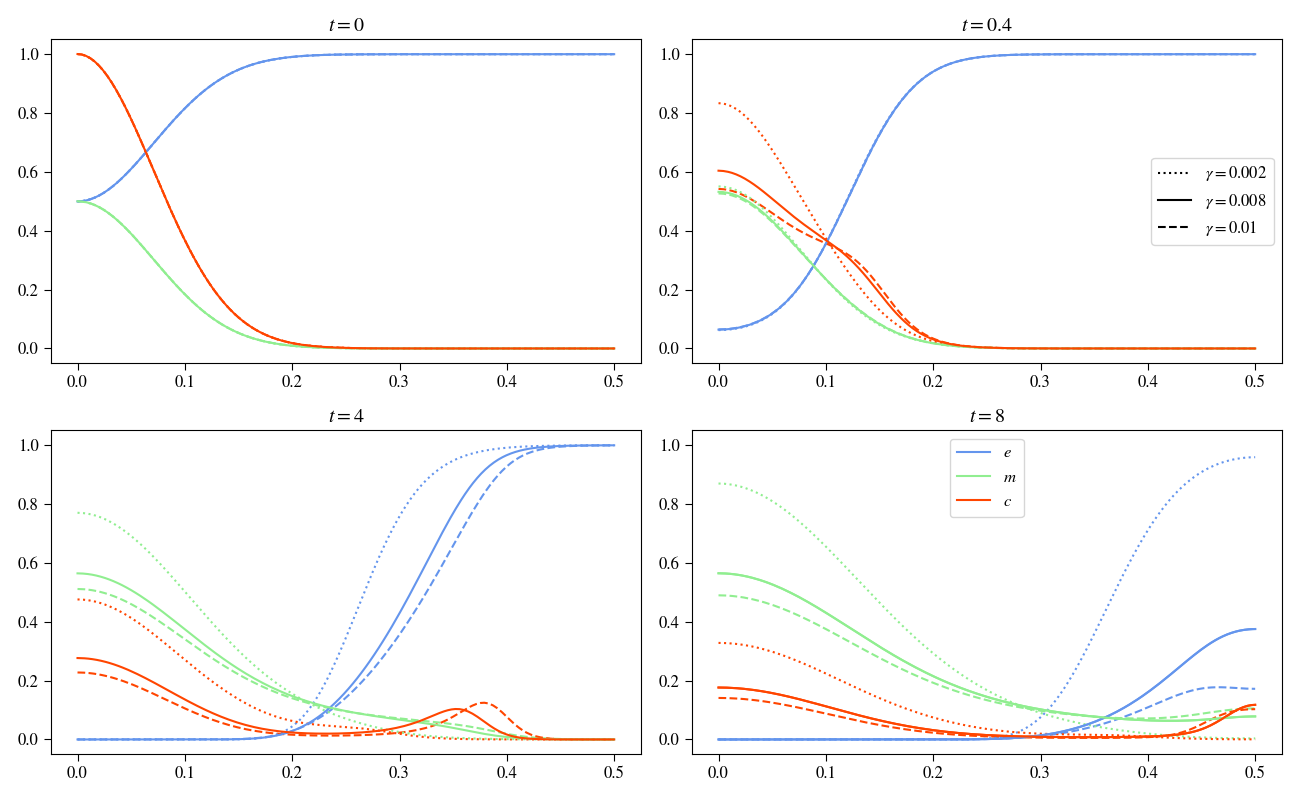
\includegraphics[width=\textwidth]{resources/images/gamma_variation.png}
    \caption{Plots show results for varying $\gamma$ whilst keeping the other parameters constant, in the images you can see the effects of $\gamma=0.01$ in the dashed curve, $\gamma=0.002$ in the dotted curve and $\gamma=0.008$ in the solid line.}
    \label{fig:gamma_variation}
\end{figure}
The experiments, described in figure\ref{fig:gamma_variation} verify the expected behaviour. After $t=4$ the solid and dashed red curves, indicating tumour concentration for the higher values for $\gamma$, have already built a lump that will in the later points in time form a secession, here we can already see that the dasehd line with the highest value for $\gamma$ has formed a larger lump than the curve for $\gamma=0.008$.The tumour density curve for $\gamma=0.002$ does not show such bevahiour. The curves for the MDE and ECM concentration still overlap at this point in time. The next image showing the simulation after $t=40$ timesteps shows that changing $\gamma$ affects also the other curves. Whilst the tumour concentration for the values of $0.008$ and $0.01$ differ slightly by the amount of density thath is left at the origin and the distance they have already invaded the surrouding tissue, the curve for the value $\gamma=0.002$ does not even show a leading edge here that is being pulled by haptotaxis into the tissue, yet it has the highest density at the origin for the $c$ curves. We can also see that with increasing $\gamma$ the invasion speed also increases. 
For the MDE curve we observe that it is still hihgest at the origin for the curves of $c$ that have lower values for $\gamma$, this only makes sense since the tumour cells produce the MDEs. For the ECM concentration we see similiar behaviour as for the MDEs, with increasing $\gamma$, the ECM is also faster decayed, again this also makes sense, since for higher values the $c$ curve curve has invaded faster and has therefore established more MDEs at farther locations away from the origin decaying the ECM.
The last image at $t=80$ confirms the observations from the previous points in time; the higher $\gamma$ the faster the invasion pace of the tumour cells and the MDEs and therefore the faster the degradation of the ECM. 
When we now take a step further and increase $\gamma$ by one potence, to $\gamma=0.1$, we can observe that the invasion pace, has gotten so high, that before finishing the simulation at $t=80$ the tumour cells have not only invaded completely up to the border regions but have also been pulled back towards the origin upon getting reflected at the border of the unit square. Also since degradation of the ECM has not kept up with the invasion pace of the tumour cells,we are left with a situation where the tumour cells have spread further than the ECM maximum and are now being pulled back inwards toward the origin again, this can be seen in figure \ref{fig:gamma_2D_plot}. Though this behaviour makes no sense from a biological perspective, due to the boundry conditions of the system reflecting the movement, it is still interessting to investigate this case, from a numerical perspective.\newline 
After already $t=20$ the tumour cells shown on the left side in this figure they have almost reached the border, looking at the ECM at this point in time we see that the highest concentration is now in the corners of the unit square. so this is where the haptotaxis is going to pull the tumour cells, this behaviour is not anymore radially symmetrical. We see in the next point in time at $t=30$ that the tumour cells do exactly this moving into the corners of the plot. Figure \ref{fig:gamma_pol_comparison} underlines this abondoning of radial symmetry, on the left side we see the plot over line configuration we used until now, the left side shows a plot over line configuration from the origin to one of the corner. After $t=20$ the images on left side imply that the tumour cells get slowly pulled back in after being reflected on the boreder, yet with a lower density, on the right side we see that tumour cells are still getting pushed outwards into regions where there is still the most ECM. In figuer \ref{fig:gamma_alt_plot} you can see the plot over line results using this alternative configuration. Up until $t=20$ everything looks like in the normal plot over line results. After this keeps going unitl hitting the border and getting reflected at $x=0.7$ which is reached between the latter two points in time. Upon getting reflected you can also see that the concentration along this line increases visibly, this is due to the tumour cells moving into the corners that have reached their borders earlier in time. As you can see this also influences the MDE and ECM concentration, with curves that are not montone since they could keep up the pace of the tumour cells invasion speed. Whilst the ECM in regions at $x=0.25$ have not decayed at $t=60$ they from a single maxima at this point, the MDEs that have been produced at the origin are at this point in time are at the same point $x=0.25$ joined by the MDEs coming from the border regions where the tumour cells there have produced them.
Where in all of the other experiments for varying $\gamma$ the tumour cells invaded at such a pace, that the produced MDE concentration in their wake was sufficiently high to degrade the ECMs to not pull the tumour cells back to the remaining ECMs later and produce montone results for both ECM and MDE concentration.
Though the intuition is met that with increasing $\gamma$ the invasion pace of the tumour cells and matrix decaying enzymes also rises, we get unexpected behaviour with the tumour cells invasion being so fast that they get reflected at the border of the unit cube and pulled into the corners and from there back in by not decayed ECM. Further increasing $\gamma$ will only increases this behaviour and make this osicilating process even faster.

\begin{figure}[h]
    \centering
    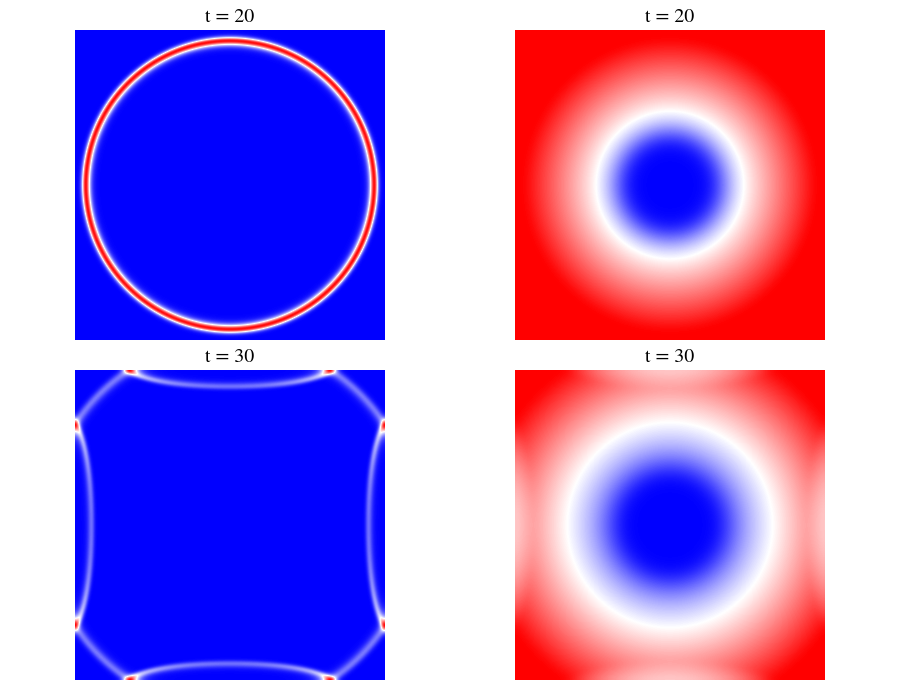
\includegraphics[width=0.9\textwidth]{resources/images/2D_plot.png}
    \caption{2D plot of variation}
    \label{fig:gamma_2D_plot}
\end{figure}
\begin{figure}[h]
    \centering
    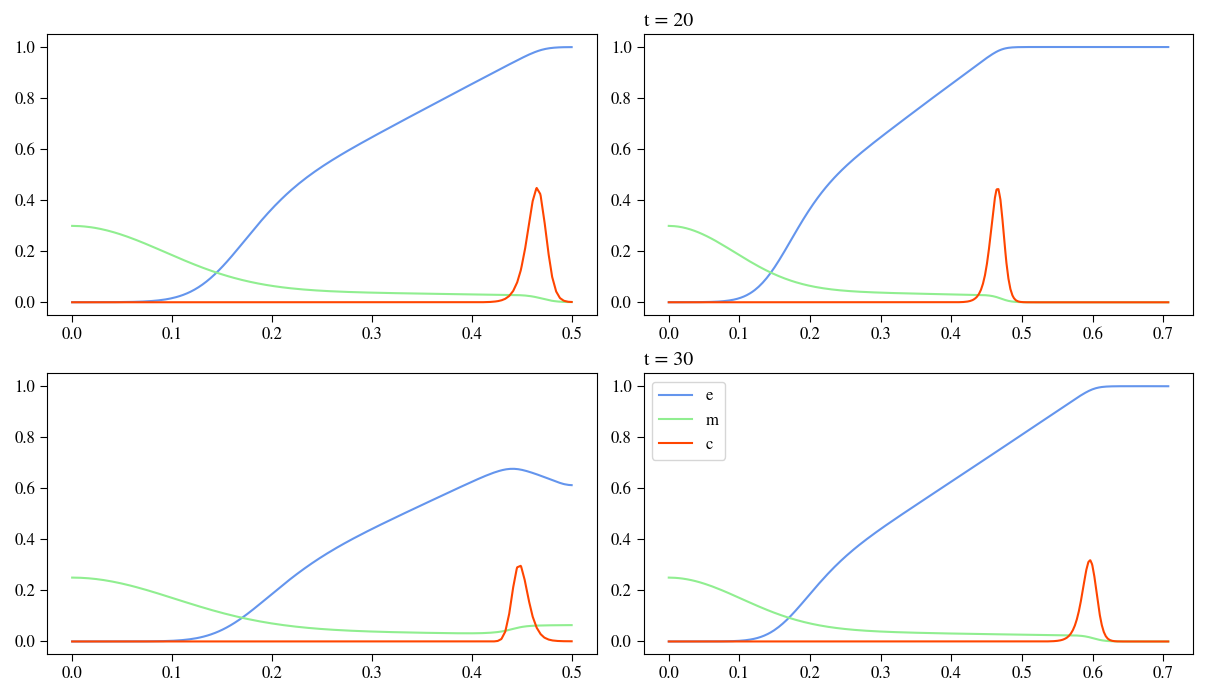
\includegraphics[width=\textwidth]{resources/images/pol_comparison.png}
    \caption{Plot OVer Line Comparison Gamma}
    \label{fig:gamma_pol_comparison}
\end{figure}
\begin{figure}[h]
    \centering
    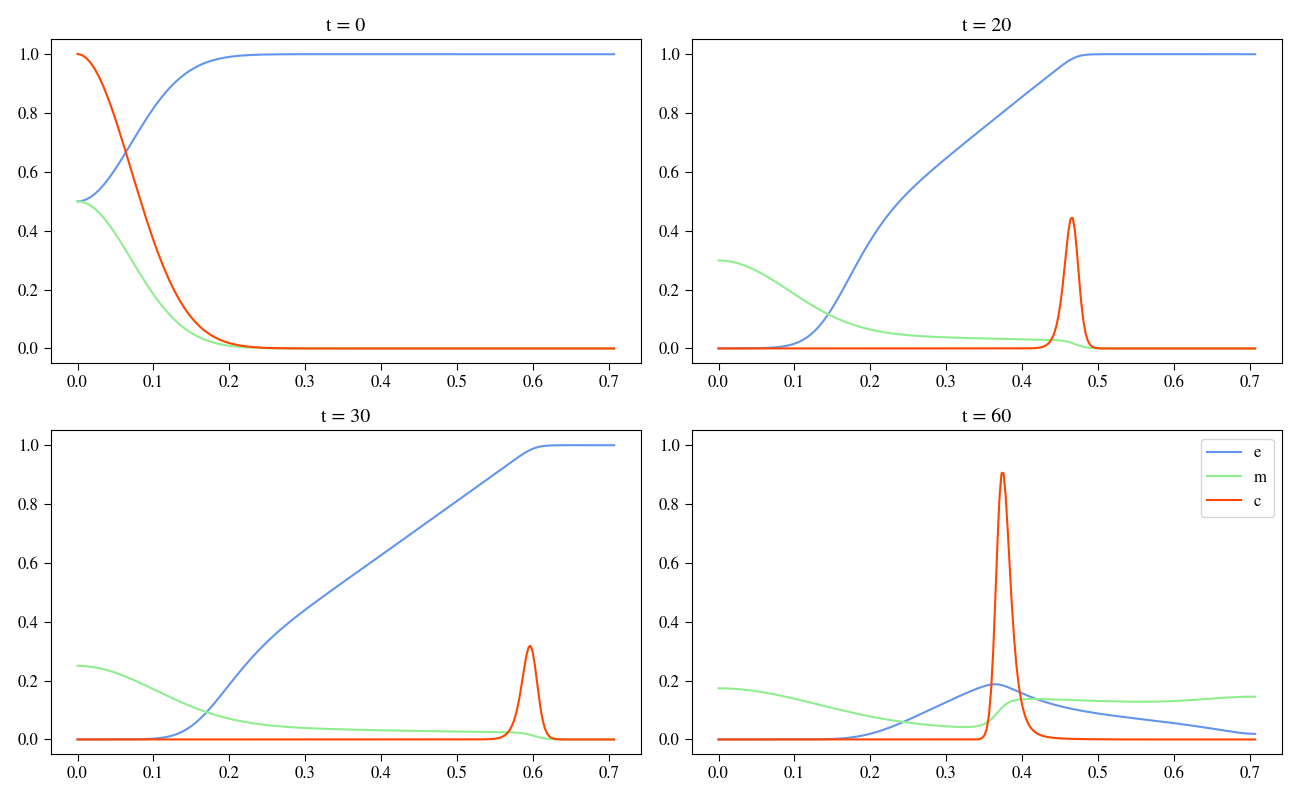
\includegraphics[width=\textwidth]{resources/images/gamma_alt_pol.png}
    \caption{gamma alternative plot over line}
    \label{fig:gamma_alt_pol}
\end{figure}

\subsubsection*{$\eta$ Variation}
\begin{figure}[h]
    \centering
    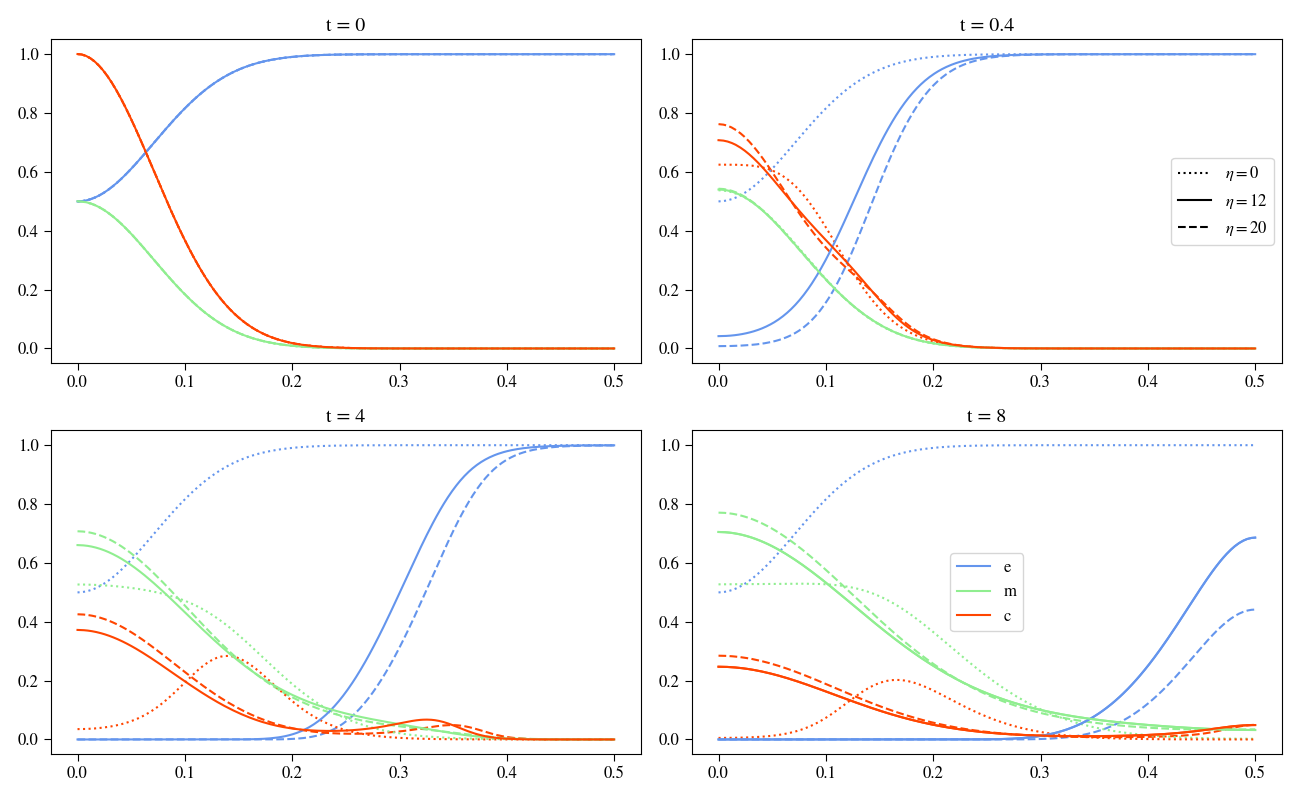
\includegraphics[width=\textwidth]{resources/images/eta_variation.png}
    \caption{Plots show results for varying $\eta$ whilst keeping the other parameters constant, in the images you can see the effects of $\eta=20$ in the dashed curve, $\eta=0$ in the dotted curve and $\eta=12$ in the solid line.}
    \label{fig:eta_variation}
\end{figure}
The parameter $\eta$ influences the degrading of the ECM, which happens faster for higher $\eta$ coefficients in regions where both MDE and ECM concentration are high. Varying this parameter may have a high impact of curves for $c$ as well, because the gradient of the ECM is a deciding factor for the effects of haptotaxis on the tumour cells, thus increasing the degradation may cause a faster shift of the ECM outwards, therefore also pulling the tumour cells faster farther out, which in turn will affect also the MDE curve.\newline
Inspecting the images in figure~\ref{fig:eta_variation} we see those assumptions met. Across all images you can see that with $\eta=0$, the dotted curves, the curve describing the ECM concentration stays constant, $\frac{\partial e}{\partial t} = 0$, this causes the tumour cell density to create no hill at the leading edge invading the tissue, since the haptotatic effect of the pull of the ECM is limited to happen with a distance of $x=0.2$. At the two later points in time the tumour cells for the experiment with $\eta=0$ take on a distribution with only one maximum located beneath where the value for $\delta c (\delta e)$ is highest, due to this point not changing much, the curve for $c$ does neither. Due to the limited motitlity of the tumour cells they doe not invade the tissue at all. The curve for the MDEs also looks much different from the basecase, after increasing intially slightly at $t=4$, the curve curve interestingly does not increase over this limit of $0.528$, with the tumour cells invading the tissue the MDEs follow with their production as well. Since the maximum of $c$ does not drastically change after $t=80$ the curve for the MDE continues increasing in this region as well, though not as strongly since the tumour cells concentration also diffuses over time. 
The solid curve describing $\eta=12$ does not strongly differ from the base case, exhibiting the expected behaviour of a stem of cells splitting off the main bulk invading the tissue at a faster rate and after $t=80$ having invaded the outer regions of the tissue as well. The curves for the MDEs and ECM follow the description of the basecase experiment. 
Increasing $\eta$ to $20$, the dashed line, the behaviour change is not so drastic comparing it to $\eta=12$. Thoug the degradation of the ECM happens twice as fast, the resulting accellerated invasion pace of the tumour cells, is not this pregnant. Interesting is that the hill at the leading edge of the tumour cells is though farther out also smaller than for the previous experiment, this might be due to the accellerated invasion pace, the tumour cells leading hill is also stretched farther. The remaining lump of tumour cells at the origin has also taken on a higher value than the experiment for the solid line, reason for this could be that with the faster degradation the effects of haptotaxis have a bigger influence on regions that are farther away from the origin, which will leave the remaining cells at the origin more subject to diffusion, because of the faster degradation the tumour cells at $x=0$ are a shorter time influenced by strong haptotatic pull, leaving more of them at the origin. Looking at the ECM concentration it has after $t=80$ as expected more decreased than previous experiments varying $\eta$. The MDE concentration has at the origin where the tumour cell concentration is higher for $\eta=20$ than for $\eta=12$ also a higher concentration, moving farther out we can also see that in those regions it is slightly lower than for the experiment with $\eta=12$, this only makes sense, since there the tumour cell density, producing the MDEs is not as strong. 
Overall we can see that with increasing $\eta$ the ECM degrading process is accellerated and also the invasion pace, with the tumour cells we can observe that due to faster invasion the remaining cells at the origin have a higher concentration as for the basecase, yet the hill at the leading edge of the tumour cells is smaller and for the MDEs they mimick this behaviour with a larger concentration at the origin as the basecase though smaller concentration at the invasion edge of haptotaxis.

\subsubsection*{$d_m$ Variation}
\begin{figure}[h]
    \centering
    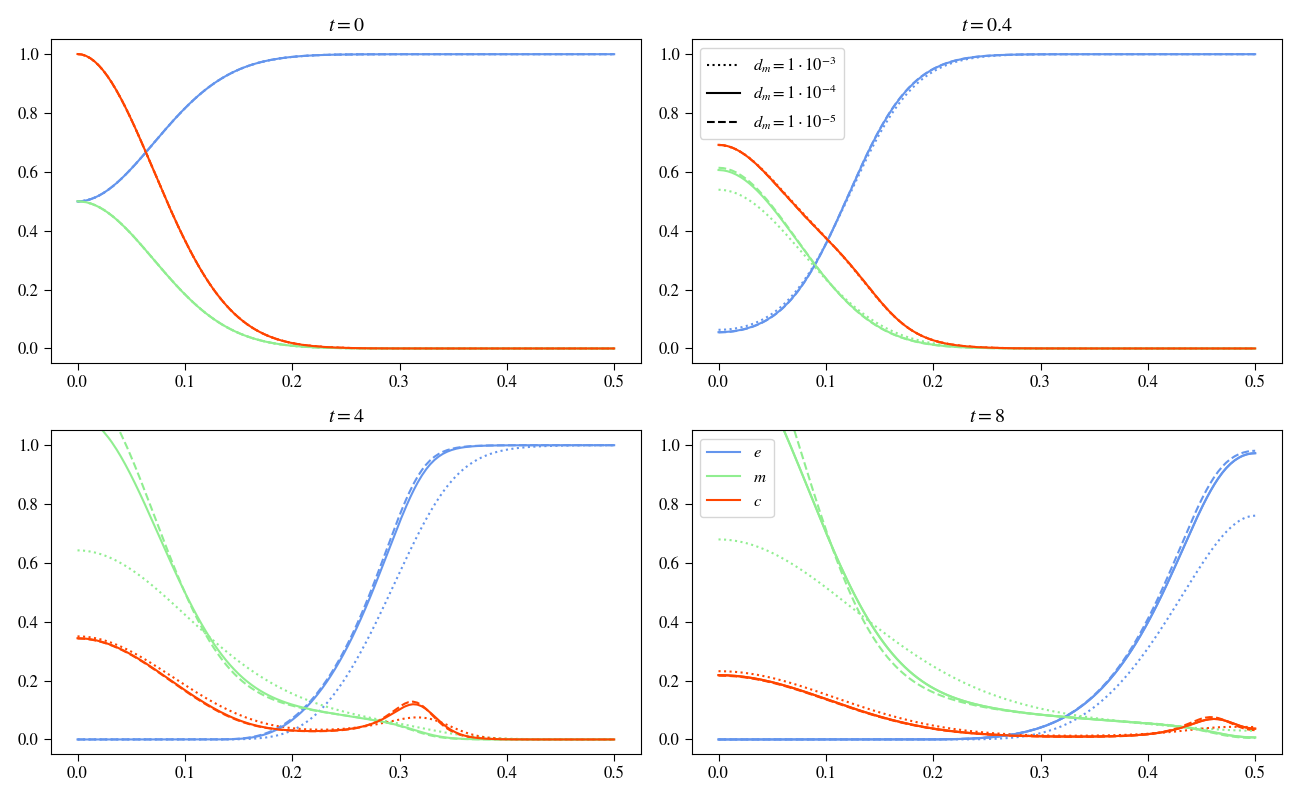
\includegraphics[width=\textwidth]{resources/images/dm_variation.png}
    \caption{Plots show results for varying $d_m$ whilst keeping the other parameters constant, in the images you can see the effects of $d_m=0.1$ in the dashed curve, $d_m=0$ in the dotted curve and $d_m=0.001$ in the solid line.}
    \label{fig:dm_variation}
\end{figure}
$d_m$ is the parameter describing the diffusion of the matrix degrading enzymes MDEs, it is influcenced by the laplacian of c, $\Delta c$. Looking at the equations we can expect with higher values for $d_m$ a faster degradation of $e$, since the MDEs can diffuse faster into the space and there isn't a high concentration of MDEs required to efficiently degrade the extra cellular matrix $e$. This will not neccessarily cause a faster invasion pace of $c$, because the ECM could be degraded more evenly and get degraded in such a way that we dont get two clearly distinctable niveaus of their concentration.
Inspecting the second image after $t=4$ we see that for $d_m=1e-3$, the solid curve, there was no movement, the curve changex only due to the production of new MDEs contributing from the tumour cells. For $d_m=0.001$ we see that its dotted curve is slightly larger at the center but moving outward it surpasses the solid curve again, the diffusion happeining mainly toward the origin at this stage. The dashed curve shows $d_m=0.1$ and in this case the MDEs have already after four timesteps taken on a constan distribution throughout space. This influences both of the other dashed curves, the tumour cells get pulled out faster and the ECM degradation is more advanced for the other two cases. For them the curves for ECM and tumour cells look nearly identical.
The next point in time $t=40$ yields interesting results. The curve of the MDEs for the case of $d_m=0$ surpasses one for the first time in the region around $x=0$, due to no outward movement and the density of tumour cells at the origin, though as the dotted ECM curve $e$ shows the degradation happens slower than for the other two cases. Interestingly the tumour cells have developed a steeper hill at the leading edge of them invading the surrouding area, due to being exposed to strong haptotactic pull for a longer time. 
Looking at the dashed line experiment, $d_m = 0.1$ we observe that the concentration of the MDEs is still constant though it has visibly risen compared to the previous image, because the produced MDEs everywhere are being distributed evenly throughout space again. As mentioned above the ECM have degraded in such a way that there are no two niveaus of them clearly distinctable due to the MDEs being already everywhere in space. This causes the effects of haptotaxis to diminish, since $\nabla e$ is decreased and therefore the tumour cells don't experience a strong pull to invade the tissue around them, resulting in such a configuration that the dashed red curve is more evenly stretched along the x-axis.
In the last image at dimensionless time $t=80$ we can observe for the dotted lined experiment, $d_m=0$ the value of the MDEs has further risen at the origin, the ECM degrading was slower than the other two and the tumour cell density of this experiment is the only one that still has a hill at its leading edge due to haptotactic pull, with the highest gradient for $e$ at this point in time. The dashed curves for the MDEs conitinue to be constantly distributed throughout space, having again clearly risen compared to the previous point in time, the blue dashed curve for the ECM is constantly zero everywhere in space, which nullifies the effect of haptotaxis on the tumour cells, leaving them only to be influcenced by diffusion, causing an more even distribution of the tumour cells throughout the space. 
As we assumed initally with improved motitlity of the MDEs the degradation happens faster, but as we also suspected the invasion does not neccessarily happen faster. Due to the ECM being complelty degraded at the last point in time the tumour cell's motiltiy is only subject to diffusion of them, which is not sufficient at this point in time, to make them invaded the border regions of the area.
	

\subsubsection*{$\alpha$ Variation}
\begin{figure}[h]
    \centering
    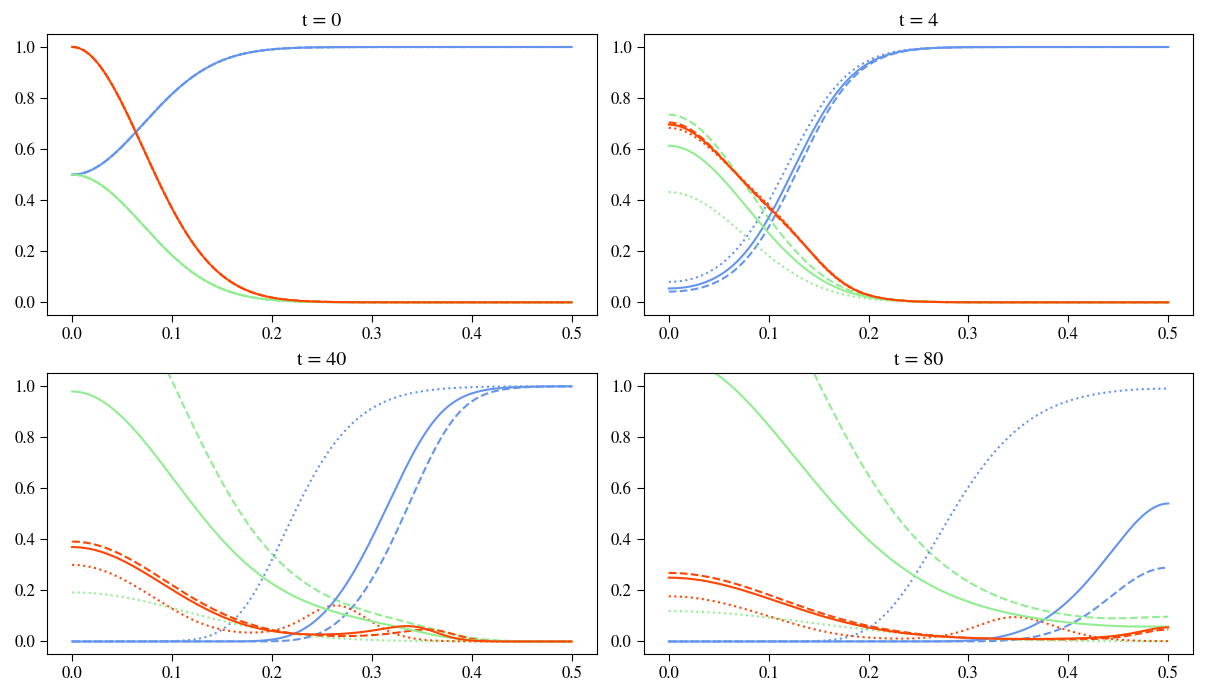
\includegraphics[width=\textwidth]{resources/images/alpha_variation.png}
    \caption{Plots show results for varying $\alpha$ whilst keeping the other parameters constant, in the images you can see the effects of $\alpha=1.0$ in the dashed curve, $\alpha=0$ in the dotted curve and $\alpha=0.6$ in the solid line.}
    \label{fig:alpha_variation}
\end{figure}
The parameter $\alpha$ influences how fast the tumour cells produce matrix decaying enzymes, looking at the system of equations it therefore depends on the concentration of tumour cells. Trying to replicate Anderson et al's experiment we already see how varying $\alpha$ affects the simulation results. Here we wil take a look at within the range of from $0.0$ to $1.0$. We can expect with growing $\alpha$ a higher concentration of MDEs which in turn will cause faster degrading of the ECM. Faster ECM degrading could mean increased invasion of the tumour cells. As we saw in the previous experiments varying $d_c$, the MDE concentration can take on values higher than one, we can also expect this here when $\alpha$ is sufficiently high.
In the second image, describing the experiments after $t=4$, we can see that the difference in the MDE curve for the different values of $\alpha$ is clear, the higher $\alpha$ the higher the concentration of the MDEs. The other curves seem not be affected as strong at this point in time though we can already see especially for th ECM concentration that the higher $\alpha$ the faster the degradation of the extra cellular matrix has already happened. The curve of the tumour cells looks almost identical for all values of $\alpha$, looking very closely we can see small deviations around $x=0$, here the previous trend is supported with higher values for $\alpha$ corresponding to also higher values for the tumour cell density. This is interesting since faster degradation as we saw varying $\eta$ results in faster invasion, but it can be explained, by the fact that with degradation happening at an increased pace, the tumour cells effect of haptotaxis also happens more strongly at regions farther away from the origin, stretching them farther out but also leaving a higher concentration at $x=0$.
The next point in time at $t=40$, shows the previous mentioned effects in an intensified way. Whilst for $\alpha=0$, dotted curves, the MDEs have no producing factor the curve flattens throughout space due to diffusion, never exceeding the value of $0.2$ for their concentration. For the ECM we see that though it has degraded visibly this happened at a slower rate than for the other experiments. The tumour cells have lowest density at the origin of the three variations, but it's hill at the leading edge has the highest volume, as explained above, due to slowed degradataion the tumour cells at the origin are a longer time subject to higher influences of haptotaxis pulling more of the cells into the surrounding tissue. The solid curves describing $\alpha = 0.6$ show that at this point in time they have almost reached a concentration of one at the center, which implies that in the following time steps the value here will exceed one. With the tumour cells have invaded farther out than in the experiment with $\alpha=0$ the ECM degradataion has also been happening faster.
Looking at the dotted lined experiment, indicating $\alpha=1.0$ the value of the MDEs at the origin has already exceeded one by far, with a value of $1,55$ at $x=0$, thus the degradation is faster, with a lower ECM curve and faster invaded tumour cell curve. 
In the last timestep we see that the MDE curve of both $\alpha=0.6$ and $\alpha=1.0$ have exceeded one. The dotted curve of the MDE shows that diffusion has distributed the MDE more evenly throughout space. At the border regions we see that the dotted curve is also the only one that has not yet degraded any ECM in this regions, whilst the dashed curve shows that there is only a little ECM concentration left to degrade. This is also shown in the curve of the tumour cells, whilst the dotted curve's peak is still somewhere around $x=0.35$ the other two curves indicate complete invasion of space. 
Our initial assumptions are correct with a faster degradation pace due to higher MDE concentration and therefore a faster invasion pace of the tumour cells. Whilst it makes from a numerical perspective sense that the concentration of MDEs can exceed one, it might make sense to introduce a finer grid or adapt the model in other ways, since judging from a continuous perspective it does not really make sense that at a certain point in space there are more than one entities, occupying this space. 

\subsubsection*{$\beta$ Variation}
\begin{figure}[h]
    \centering
    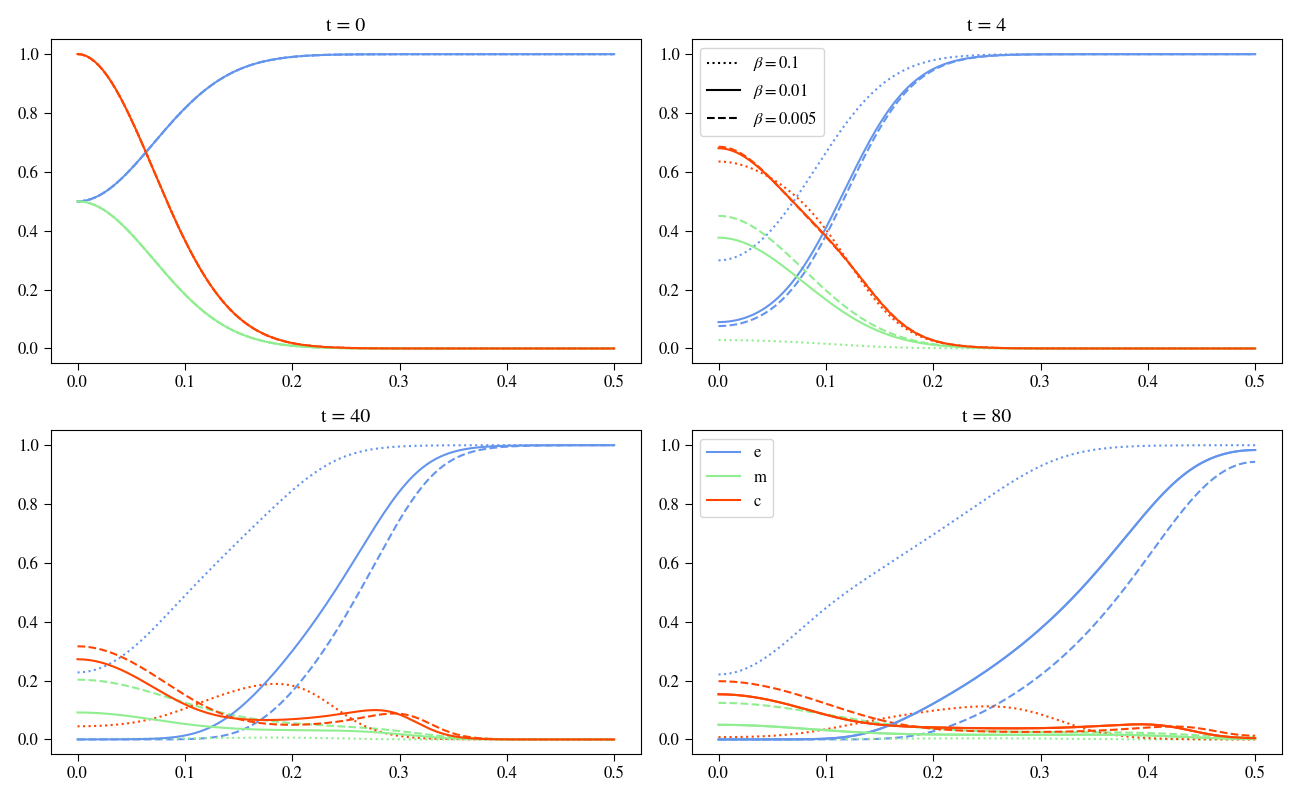
\includegraphics[width=\textwidth]{resources/images/beta_variation.png}
    \caption{Plots show results for varying $\beta$ whilst keeping the other parameters constant, in the images you can see the effects of $\beta=0.005$ in the dashed curve, $\beta=0.1$ in the dotted curve and $\beta=0.01$ in the solid line.}
    \label{fig:beta_variation}
\end{figure}

Looking at a variaton of $\beta$, in figure~\ref{fig:beta_variation} which is the parameter describing decay of the MDEs, we can assume that with varying $\beta$ the MDE curve will be lower, influcencing the ECM degrading process and therefore also the invasion pace. Since all previous experiments assumed a value of $\beta=0$ we are going to look for a value here that is neither too high to distort the whole simulation nor a value too low to have no effect on it. We first of all needed to determine a range in which to experiment. Starting with a range of values between $0.1$ and $1.0$, since this is the range $\alpha$ yields reasonable results in and $c$ and $m$ are in the same scale regarding their values, we counter-intuitively saw that those values were much too high. Even for $\beta=0.1$, shown in the dotted curve, the MDEs are almost completely decayed after only $t=4$, leaving only a small portion of MDEs at the origin due to the production from the tumour cells.
This makes the ECM degradation process visibly slower and makes the tumour cells a longer time subjected to high effects of haptotaxis, causing to only develop one hill, visible in the red dotted curve.
Looking at the different points in time we can see that though the dotted green MDE curve is nearly everywhere zero we see that degradation still happens visibly and due to the longer exposition on haptotaxis on bigger portions of tumour cells this one lump of cells is being pull through space.
Decreasing to $\beta=0.01$ we see that the for the solid lines in figure~\ref{fig:beta_variation} the MDE concentration takes on higher values througout the points in time. The tumour cells density show again a distinction between the effects of diffusion and haptotaxis, resulting in a two distinctly different lumps with different maxima and ECM degrading resembles most of the previous experiments, though the gradient here is not as steep especilly in the last point in time. 
Further decreasing $\beta$ to $\beta = 0.005$ we see the effects observed in $\beta=0.005$ increase, with a higher concentration of MDEs throughout space and time, and also a faster degradation process. The tumour cells for the dashed curve split into mainly two areas, where the density at the origin is higher than the solid line curve for $\beta=0.01$, and have furhter invaded into the tissue, with a lower density at the leading edge.
Having only one refrence value in Kolev et al's\cite{Kolev2010} paper with $\beta=0.07$ we experimented with this value though saw as we did for $\beta=0.1$ that it was too high distroting the results too strongly, we will further use a range from $0.001$ to $0.01$ to experiment in for $\beta$ as seen in the experiments from figure~\ref{fig:beta_variation}. Here our assumptions were also met, concluding that with rising $\beta$ values the ECM degradation slows down, this also causing the invasion pace of the tumour cells to diminish.

\subsubsection*{Cross Variation}
Having done all those experiments it will be interesting to cross vary both effects on the same variable and countering or increasing effects.

\subsubsection*{$d_c - \gamma$ Variation}
\begin{figure}[h]
    \centering
    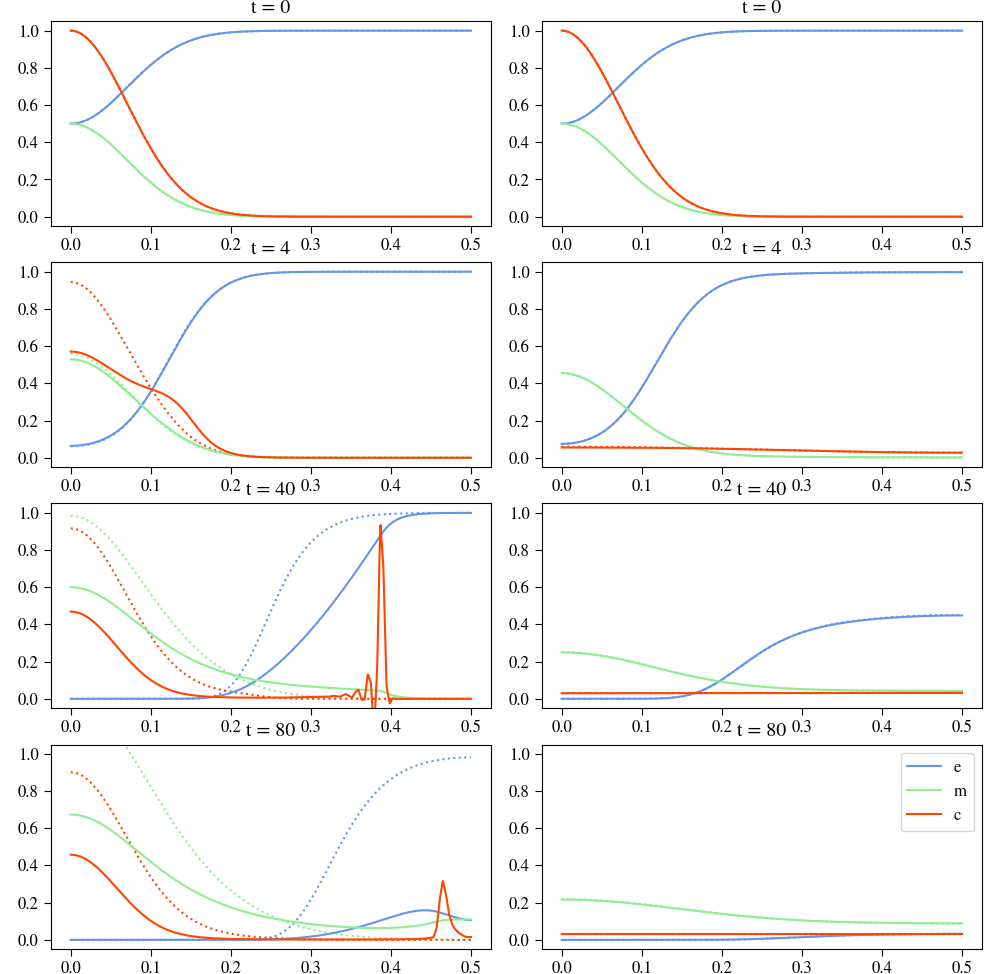
\includegraphics[width=0.85\textwidth]{resources/images/dc_gamma_variation.png}
    \caption{Plots show results for varying both $d_c$ and $\gamma$ whilst keeping the other parameters constant, in the images on the left $d_c$ is set to $d_c=5e-5$ with the solid line showing $\gamma = 0.01$ and the dotted line $\gamma=0.001$ on the right $d_c$ is set to $d_c=1e-1$ with the solid line showing $\gamma = 0.01$ and the dotted line $\gamma=0.001$.}
    \label{fig:dc_gamma_variation}
\end{figure}

Having set $d_c=5e-5$ and $\gamma=0.001$ we see no secession of the tumour cells, the effects of haptotaxis are too small leaving the tumour cells only subject to diffusion which results in an even distribution process over time, which also causes a slower invasion pace. Because the tumour cells stay in a lump with its maxima at the origin $x=0$ the MDEs also take on their maximum there, moving farther out they also distribute very evenly. This staying with values around the origin of the MDEs causes a slower ECM degradation. Increasing $\gamma=0.01$ we see that the effects of haptotaxis are now pregnantly visible with a very sharp maxima seen at $t=40$, which equals the maxima of the remaining tumour cell lump at $x=0$. Stronger influence of haptotaxis leads to a faster invasion pace of the tumour cells into the tissue and allowing to create matrix degrading enzymes in their wake, causing a more even distribution compared to $\gamma=0.001$ and also a faster ECM degrading process. 
Looking at the right side of the plot ~\ref{fig:dc_gamma_variation} we see the results for $d_c=1e-1$ here for both $\gamma$ values diffusion overshadows the effects of haptotaxis completely, with after already $t=4$ having a constant distribution of tumour cells throughout space. Due to this fast spread of tumour cells, the MDEs are also produced evenly throughout space, and an even faster ECM degradataion. 

\subsubsection*{$d_m - \eta$ Variation}
\begin{figure}[h]
    \centering
    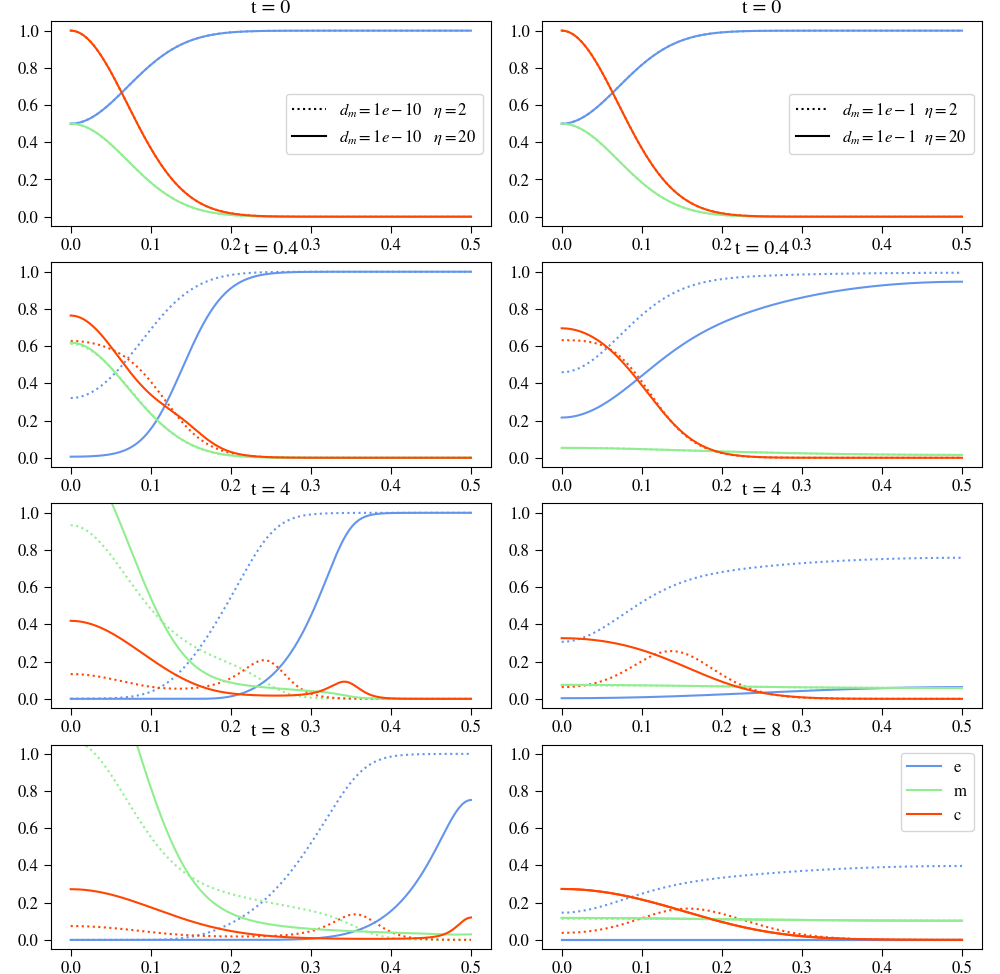
\includegraphics[width=0.85\textwidth]{resources/images/dm_eta_variation.png}
    \caption{Plots show results for varying both $d_m$ and $\eta$ whilst keeping the other parameters constant, in the images on the left $d_m$ is set to $d_c=1e-10$ with the solid line showing $\eta = 2$ and the dotted line $\eta=20$ on the right $d_m$ is set to $d_m=1e-1$ with the solid line showing $\eta = 2$ and the dotted line $\eta=20$.}
    \label{fig:dm_eta_variation}
\end{figure}

Looking at low values for both $d_m$ and $\eta$ in the figure~\ref{fig:dm_eta_variation}, the dotted curve in the left column, we see that slow diffusion of the matrix degrading enzymes and slow degradation of the extra cellular matrix causes the tumour cells to only develop one lump that invades space, due to stronger haptotatic exposition to a slower degraded ECM, to create larger values for $\nabla (c \nabla e)$, this is also observable for the higher diffusion values and lowwer ECM degrading factors. Having this single lump with a lower maxima and larger length causes the MDEs to produce more evenly farther away from the origin. The low value for the ECM degrading factor results in an overall slower ECM degradation. Looking on the solid line on the left colum we see that increasing $\eta$ enables the tumour cells to develop two hills, one staying at $x=0$ and one invading space by haptotatic pull. Due to a higher density of tumour cells at the origin the MDEs produced there exceed a value of one and ECM degrading happens faster due to first the higher coefficient but also because of a faster invasion pace of matrix degrading enzymes, due to faster invasion of the tumour cells. Increasing $d_m$ to $d_m=1e-1$ causes the MDE concentration to flatten throughout space, taking on a constant distribution in space for one point in time, neglecting the values for $\eta$. Though $\eta$ still has an influence on both tumour cell density and ECM concentration. We see that, as previously mentioned, for $\eta=2$ the degrading happens so slow that the tumour cells form only one lump invading the tissue, with its maxima travelling along the x-axis. In contrast to this for $\eta=20$, we also see only one lump develop though this one stays with it's maxima at the origin. For $\eta=20$ we see that after $t=40$ the ECM has almost completly degraded, making the formation of a secondary lump invading the tissue not possible due to too low haptotatic pull. 

\subsubsection*{$\alpha - \beta$ Variation}
\begin{figure}[h]
    \centering
    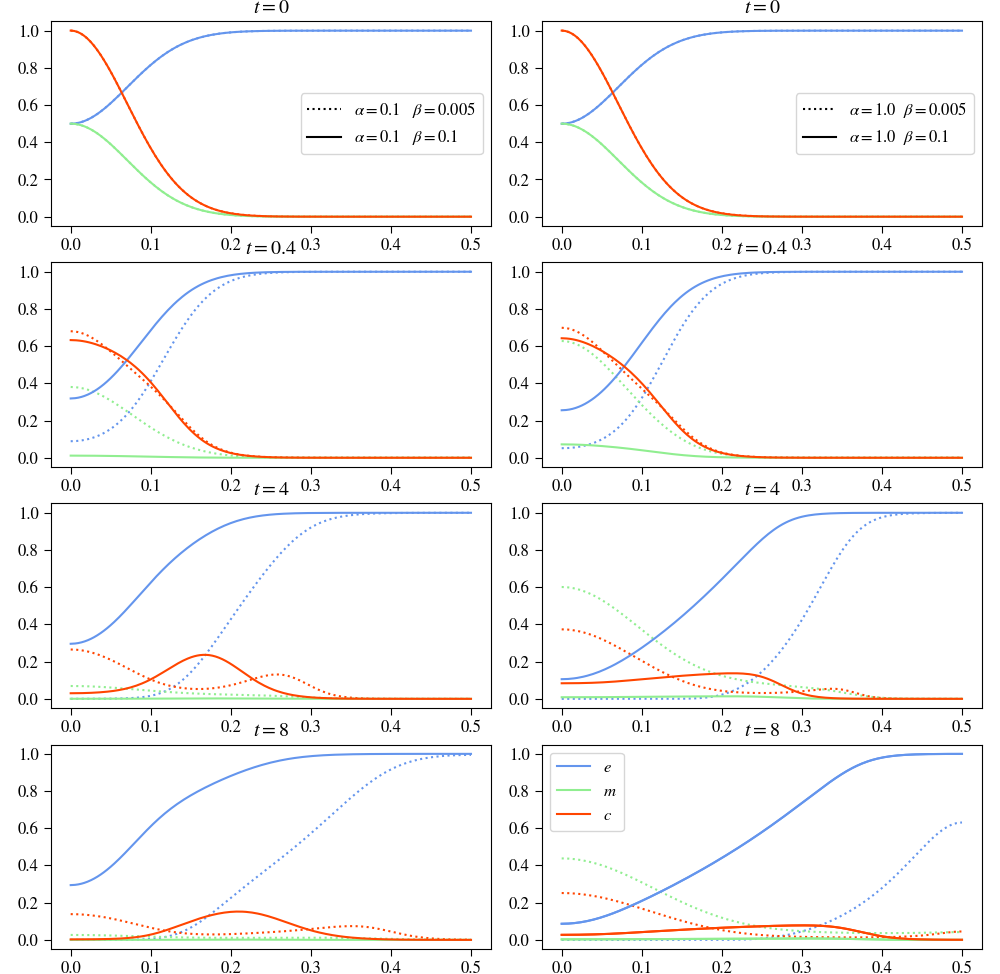
\includegraphics[width=0.85\textwidth]{resources/images/alpha_beta_variation.png}
    \caption{Plots show results for varying both $\alpha$ and $\beta$ whilst keeping the other parameters constant, in the images on the left $\alpha=0.1$ with the solid line showing $\beta = 0.005$ and the dotted line $\beta=0.1$ on the right $\alpha=1.0$ with the solid line showing $\beta = 0.005$ and the dotted line $\beta=0.1$.}
    \label{fig:alpha_beta_variation}
\end{figure}

Looking at figure~\ref{fig:alpha_beta_variation} we see experimental results varying both $\alpha$ and $\beta$. For low MDE production but also low MDE decay we can see that the curve for the MDEs is still visible at up to $t=40$, at $t=80$ it is zero. We see that first the ECM degrading happens faster than for high $\beta$ values and therefore the tumour cells develop two lumps with one invading the tissue the other staying at $x=0$. The maxima for both lumps is lower than in previous experiments, though the cells seem to be more evenly distributed in between the two lumps. Increasing $\beta=0.1$ the MDE curve seems to be zero after already $t=$ and stays there until the end of this experiment. This low concentration of MDEs casuses a slower ECM degrading process and therefore leads the tumour cells to only develop one lump, invading the space, with its maxima moving at the center of this lump. For $\alpha=0.1$ both values for $\beta$ have proven to be to high, decaying the matrix degrading enzymes too fast to keep up with production.
On the other hand increasing $\alpha$ to $1.0$ and keeping $\beta=0.05$, we see that production outweighs decay, with at the end of the experiment the MDEs still have a concentration of about $0.4$ at $x=0$. For this experiment we seee that the tumour cells develop two lumps indicating that diffusion and haptotaxis effects are also in some balance, and ECM degradation seems to resemble due to similiarities with the basecase for the MDE curve, also the ECM degradation of the basecase experiment.
Increasing both $\alpha$ and $\beta$ we see in the solid line of the right column of figure~\ref{fig:alpha_beta_variation} that decay outweighs production again, after $t=4$ we can only see a small remaining portion of matrix degrading enzymes at the origin. This causes a slower ECM degradataion and therefore to forming only one lump of tumour cells, due to too strong effects of haptotaxis, though this singular lump is streched flat along the x-axis.

\subsubsection*{$d_m - \alpha - \beta$ Variation}
\begin{figure}[h]
    \centering
    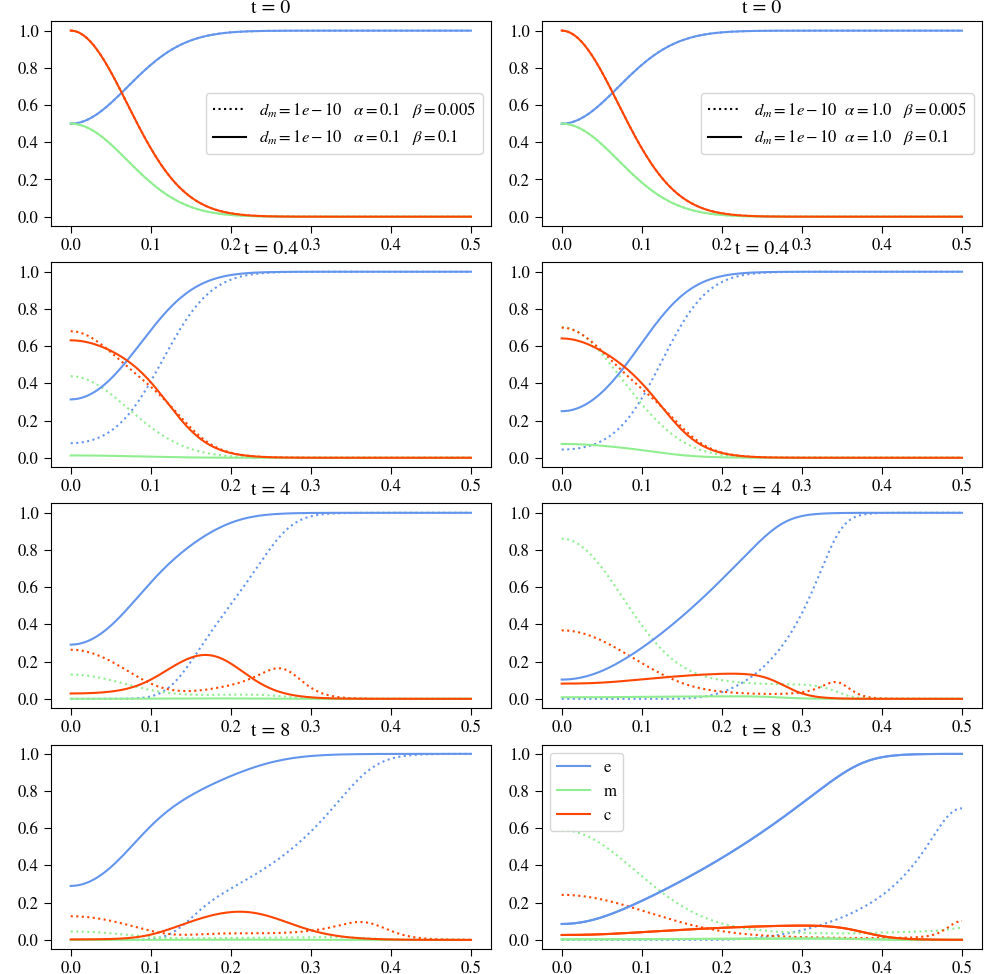
\includegraphics[width=0.85\textwidth]{resources/images/dm_alpha_beta_variation_1.png}
    \caption{Plots show results for varying both $\alpha$ and $\beta$ whilst keeping the other parameters constant, in the images on the left $\alpha=0.1$ with the solid line showing $\beta = 0.005$ and the dotted line $\beta=0.1$ on the right $\alpha=1.0$ with the solid line showing $\beta = 0.005$ and the dotted line $\beta=0.1$.}
    \label{fig:dm_alpha_beta_variation_1}
\end{figure}
\begin{figure}[h]
    \centering
    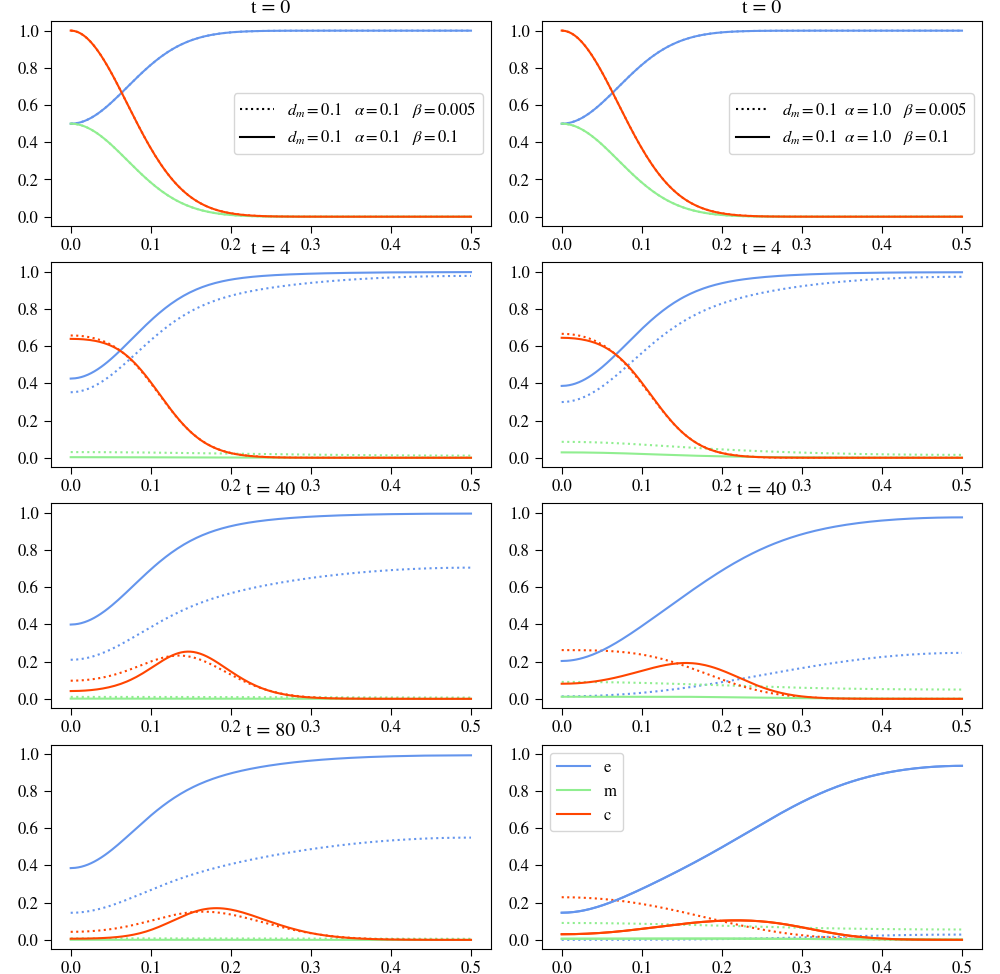
\includegraphics[width=0.85\textwidth]{resources/images/dm_alpha_beta_variation_2.png}
    \caption{Plots show results for varying both $\alpha$ and $\beta$ whilst keeping the other parameters constant, in the images on the left $\alpha=0.1$ with the solid line showing $\beta = 0.005$ and the dotted line $\beta=0.1$ on the right $\alpha=1.0$ with the solid line showing $\beta = 0.005$ and the dotted line $\beta=0.1$.}
    \label{fig:dm_alpha_beta_variation_2}
\end{figure}

Experimenting with all parameters regarding the equation for the matrix degrading enzymes required to split the results into two figures,~\ref{fig:dm_alpha_beta_variation_1} and ~\ref{fig:dm_alpha_beta_variation_2}, due to clarity reasons. 
We are first going to take a look at the results in figure~\ref{fig:dm_alpha_beta_variation_1}, to see the effect of a decreased diffusion coefficient for the MDEs. We observe that with having $\alpha =0.1$ and $\beta=0.005$ the ECM degradation happens faster due to having a higher MDE concentration, because of lower MDE decay. Which also increases the seperation of the effects of haptotaxis and diffusion on the tumour cells, seperating them into two lumps, one being pulled them along the ECM faster into the tissue the other staying at the origin. Though the MDE concentration diminishes over time we can still see little remaining concentration at the end at $t=80$. Increasing $\beta$ diminishes the MDE concentration sharply, slowing down the ECM degrading process, which increases the effect of haptotaxis over diffusion to pull all of the tumour cells away from the origin to invade the tissue as one lump though at a slower pace. Over time we can see that as expected the tumour cell density's maximum is located approximately right below where $\nabla (c \nabla e)$ is highest. \newline
Looking at the experiments with higher $\alpha$ values we can see that for lower $\beta$ values the MDE concentration oscilates up and down over time, which indicates that with this configuration of $\alpha$ and $\beta$ values we found a balancing point. For higher $\beta$ values we cannot observe this balance, since in this case the MDEs have nearly decayed after $t=40$. Having such differences in the MDE concentration we can also see big differences in the ECM concentration. Here we see that as expected with $\beta=0.005$ the ECM degradation happens a lot faster than having $\beta=0.1$. These changes in the ECM concentration also affect the tumour cell density. Like in the experiments with $\alpha=0.1$ the results for having higher $\beta$ lead to only one lump invading the tissue with a more even distributed density along the x-axis, whereas lower $\beta$ values made the diffusion and haptotaxis differentiable forming two lumps one to stay at the origin, one to invade the tissue outwards.\newline 
Next we are investigating how changing $d_m$ as well will affect the system, looking at figure~\ref{fig:dm_alpha_beta_variation_2}. First of all it is to say that as with varying $d_m$ only the diffusion here is also strong enough to in most cases completely evenly distribute the matrix degrading enzymes in all of the space after already the fourth step in time. \newline 
On the left side we see the experiments with low $\alpha$ values and see that less decay of the MDEs leads to slower ECM degradataion. Due to the very even distribution of the MDEs we see for both cases a more evenly degradation of the ECM, with overall lower gradients. This results in a longer exposition of haptotatic effects on the tumour cells to form only lump invading the tissue with a moving maximum, though for a lower $\beta$ factor we see that a larger is staying at the origin since the haptotatic pull here is weaker due to having also a more evenly distributed tumour cell density.\newline 
Looking at the right side of figure ~\ref{fig:dm_alpha_beta_variation_2} we see with increased $\alpha$ the results regarding the tumour cell density differ strongly. Whereas on the left side we saw that there was always one lump to invade the cells with its maximum moving below where $\nabla(c\nabla e)$ is strongest, we see that for low $\beta$ the lump of tumour cell stays with its core at the origin at $x=0$, where also its maximum is, and invades the tissue with no leading edge. This shows the effect of a both sufficiently fast and efficient degradation of extra cellular matrix. Here we see diffusion as the main factor for the movement of the tumour cells since the haptotatic pull is very low, due to small gradients of $e$ only. For the other curves we can observe that as before with rising $\beta$ the ECM degradation pace slows down, in the last point in time the difference $\beta$ causes is pregnantly visible with for low $\beta$ the ECM has been degraded completely but for high $\beta$ there is still a considerable concentration. Looking at the MDE concentration we can also see clear differences regarding the influence of the diffusion on the MDE decay. Though the MDE concentration with high diffusion is more evenly distributed, its overall volume in space is clearly lower than for low diffusion terms, with same $\alpha$ and $\beta$ configuarations.



\subsection{Two dimensional Results with Proliferation}
In this section we are going to inspect the updated system, consisting of equation ~\ref{eq:6} to ~\ref{eq:10}, to describe the effects of tumour cell proliferation and extra cellular matrix renewal processes.

\subsubsection*{Basecase Analysis}

Here is also makes sense to establish a basecase to compare the following parameter analysis resulst against. For this we used the values $\mu_1= 0.1$ and $\mu_2=0.5$ according to the only experiment found for this system of equations in the paper of Kolev et al. \cite{Kolev2010}.\newline
Comparing this new basecase to our initial model's basecase we can see the influences of both $\mu_1$ and $\mu_2$, as for the tumour cell density curve is visibly higher than without proliferation, causing a higher production of matrix degrading enzymes, which would lead to faster ECM degradation, though this is countered by the renewal factor $\mu_2$ causing the ECM concentration to be higher at the end, at $t=80$, than in the initial basecase experiment.

\begin{figure}[h]
    \centering
    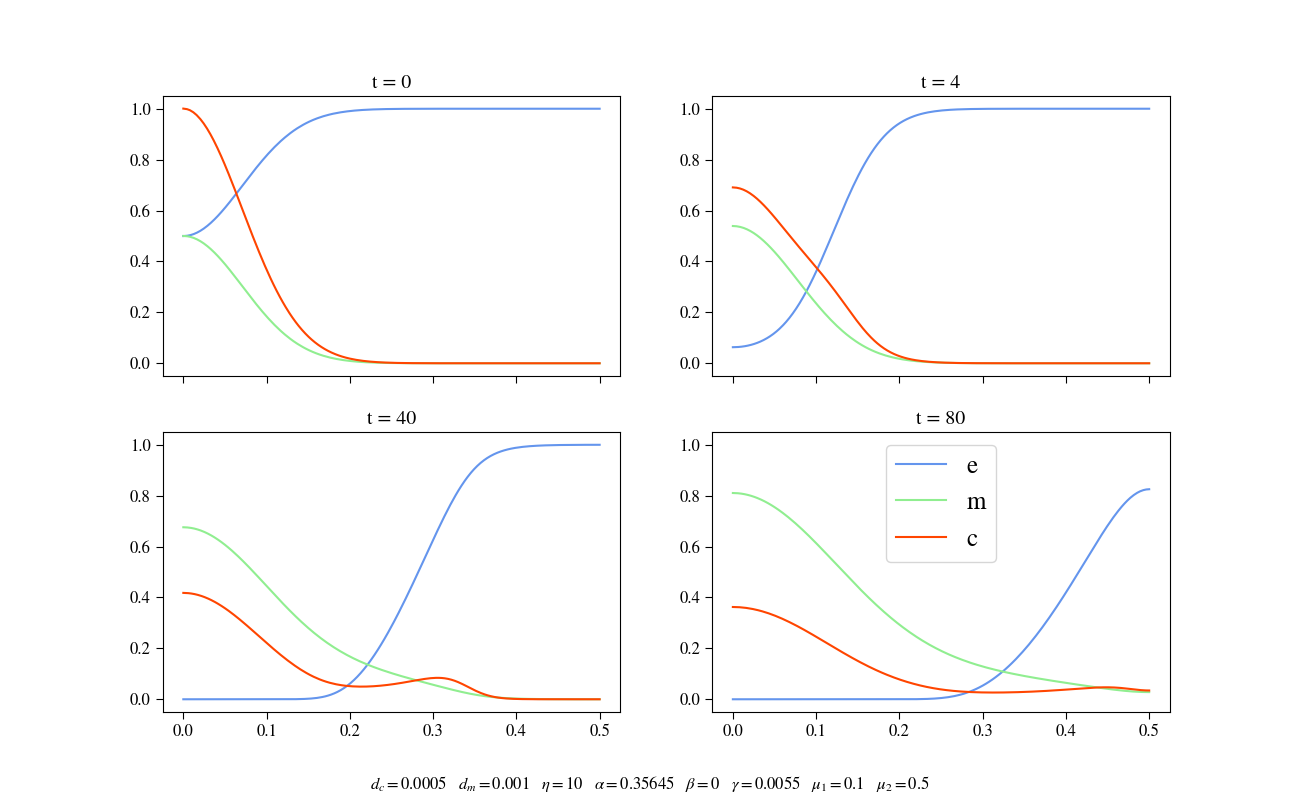
\includegraphics[width=\textwidth]{resources/images/basecase_proliferation.png}
    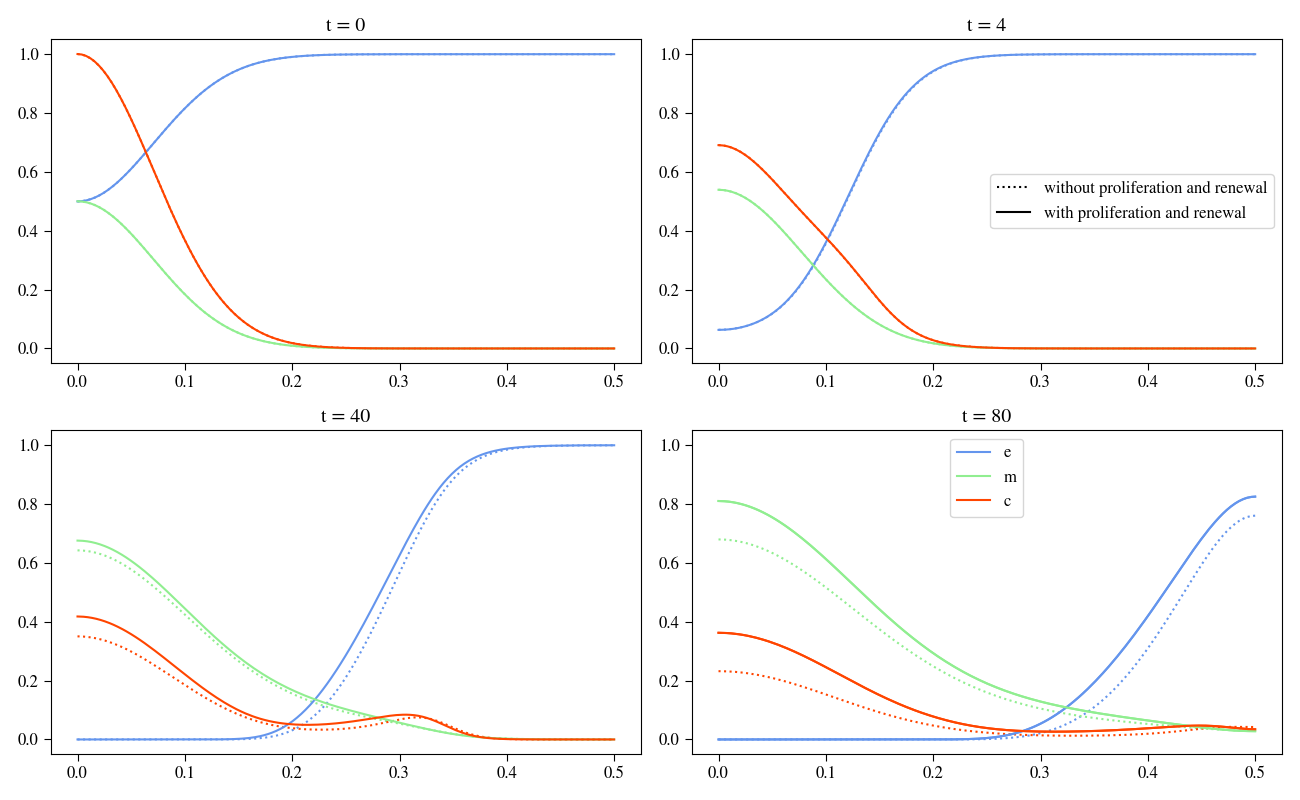
\includegraphics[width=0.8\textwidth]{resources/images/basecase_comparison.png}
    \label{fig:prolif_basecase}
    \caption{Describing the updated basecase, in the image above only the updated basecase is plotted, below it is compared to the initial basecase.}
\end{figure}





\subsubsection{Parameter Analysis}

For the Parameter Analysis of the model with proliferation and renewal we are focusing on comparing the results of the updated model with the results produced by the model without renewal and proliferation, this will point out again the influence of $\mu_1$ and $\mu_2$ on the system. 

\subsubsection*{$d_c$ Variation}
\begin{figure}[h]
    \centering
    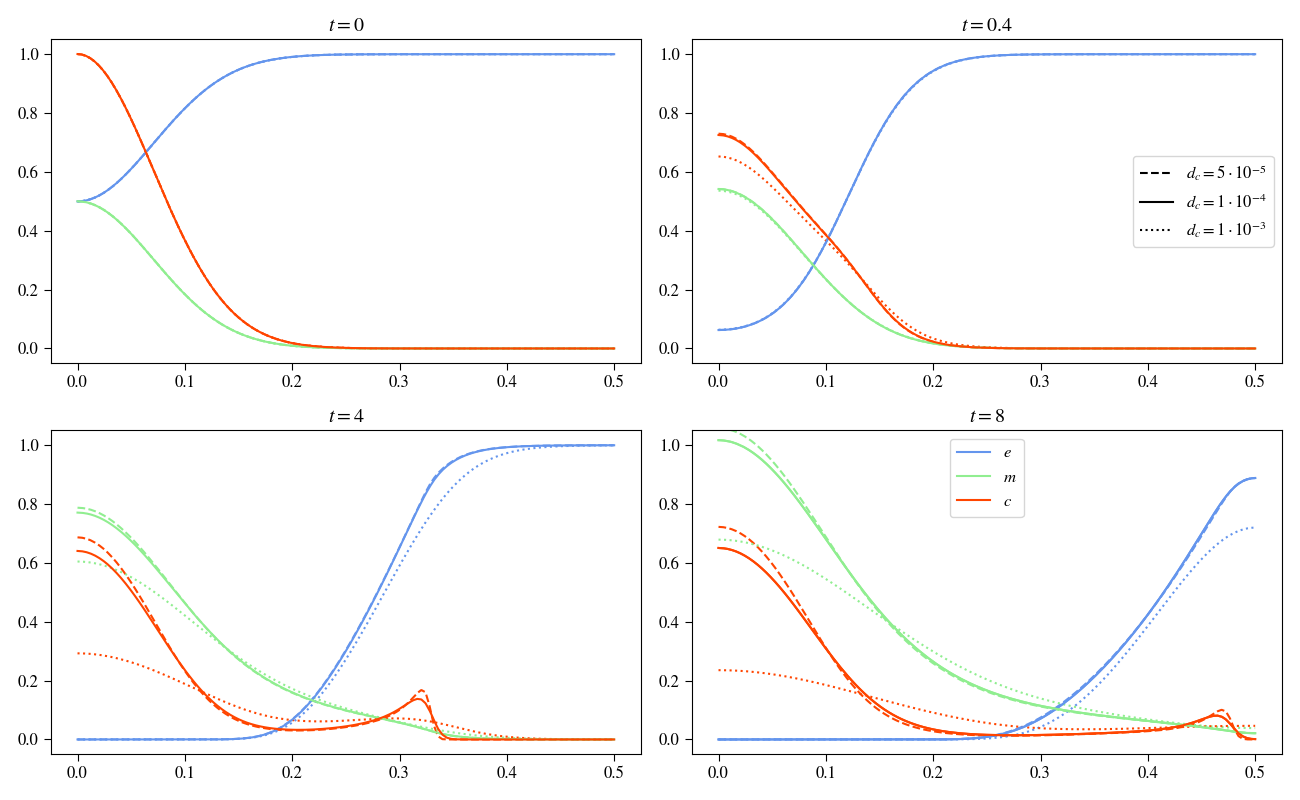
\includegraphics[width=\textwidth]{resources/images/prolif_dc_variation.png}
    \caption{Plots show results for varying $d_c$ whilst keeping the other parameters constant}
    \label{fig:prolif_dc_comparison}
\end{figure}

Varying $d_c$ with proliferation terms, we see the same effects as without proliferation. Higher values for $d_c$ cause a stronger influence of diffusion and a weaker for the haptotaxis, which leads to a curve with less or none of a leading edge invading the space, but to a faster rather constant distribution throughout space. The MDE concentration follows this behaviour, depending on its production on the tumour cell density distribution in space and the ECM is decayed faster, the faster the tissue is invaded, thus the higher the diffusion factor is. Comparing them we see little differences, only tumour cell density and ECM are raised a little in each plot due to the renewal and proliferation factors, which in turn also causes a higher MDE concentration, due to higher tumour cell densities. 


\subsubsection*{$\gamma$ Variation}

\begin{figure}[h]
    \centering
    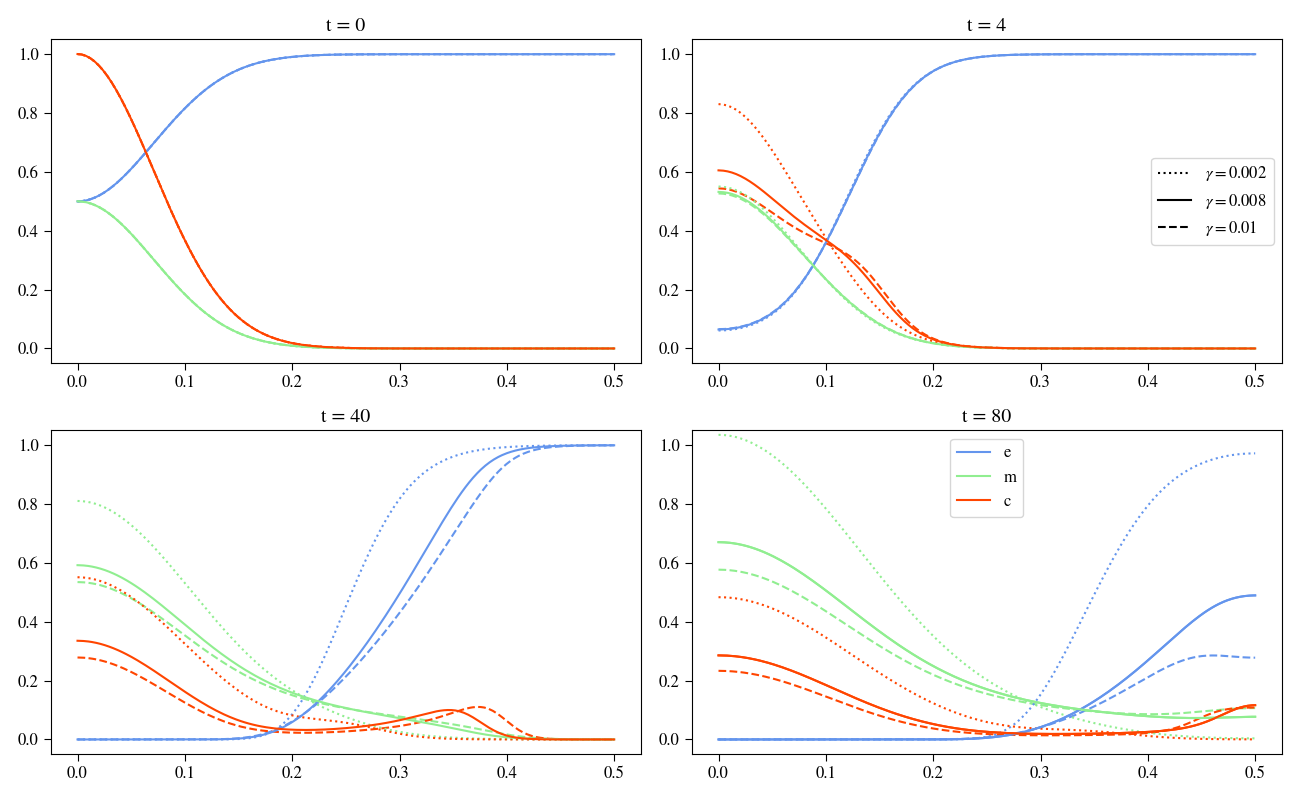
\includegraphics[width=\textwidth]{resources/images/prolif_gamma_variation.png}
    \caption{Plots show results for varying $\gamma$ whilst keeping the other parameters constant.}
    \label{fig:prolif_gamma_variation}
\end{figure}

When we look at $\gamma$ we also can see the same effects as the model without proliferation shows, with the adjustments as varying $d_c$, with raised curves for all variables. Increasing $\gamma$ means increasing haptotaxis effects, pulling the tumour cells stronger towards the extra cellular matrix molecules, which causes a faster invasion pace and also a higher density of tumour cells invading the tissue, but a lower staying at the centere at $x=0$. This also means that the ECM degrading process happens faster and the MDEs are more evenly distributed through space the higher $\gamma$ is. As mentioned above the same effects come in this experiment, introducing proliferation and renewal, with higher values for tumour cell density, MDE and ECM concentration especially at the later points in time clearly depictable. It is interessting to observe that though introducing a renewal factor for the extra cellular matrix, the proliferation of the tumour cells causes a faster production of matrix degrading enzymes, which makes the system produce nearly the same results as without proliferation and renewal concerning the ECM concentration, still  it is to say that introducing the renewal of the ECM results in overall slightly higher concentrations of it.

\subsubsection*{$\mu_1$ Variation}
\begin{figure}[h]
    \centering
    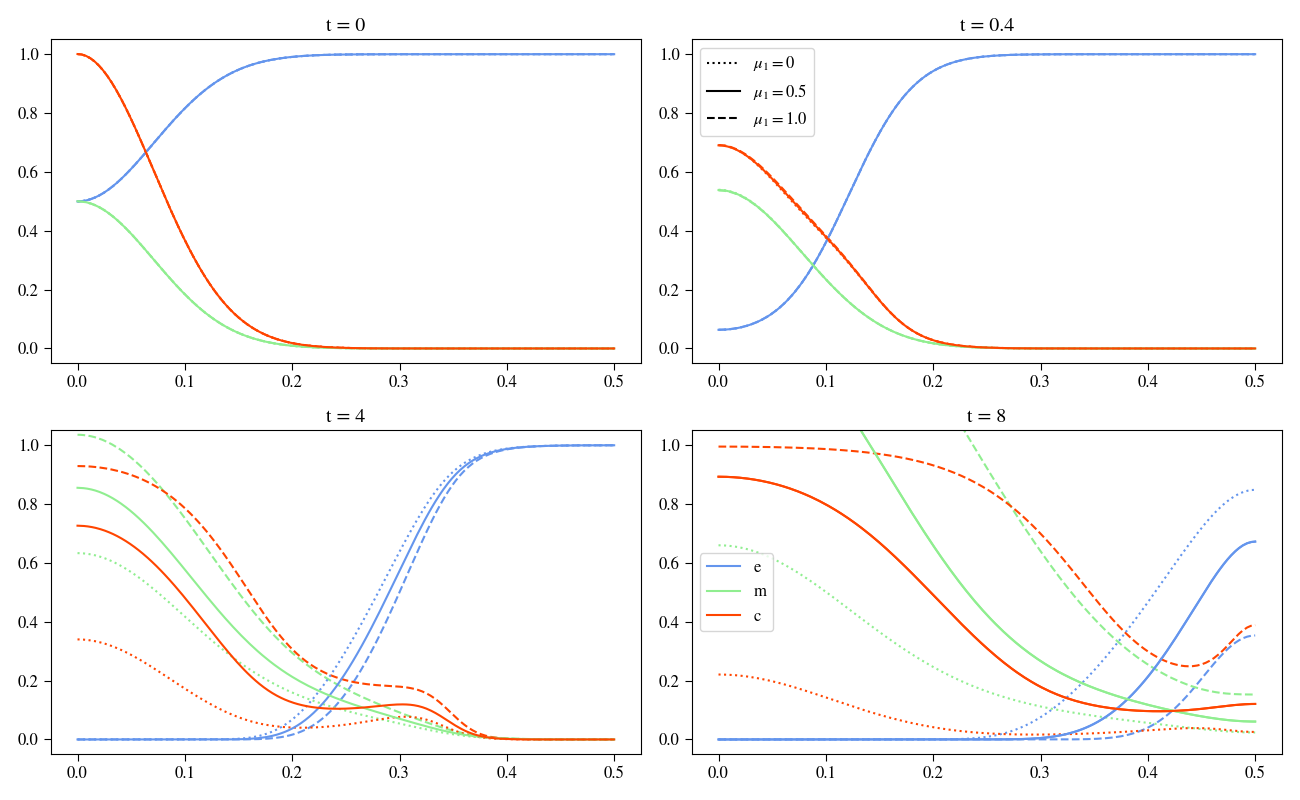
\includegraphics[width=\textwidth]{resources/images/prolif_mu_1_variation.png}
    \caption{Plots show results for varying $\mu_1$ whilst keeping the other parameters constant.}
    \label{fig:prolif_mu_1_variation}
\end{figure}

The parameter $\mu_1$ describes the proliferation of the tumour cells, with assuming logisitcal growth in this term, being limited by the already present ECM molecules and tumour cells. We see that with varying $\mu_1$ the other curves are also strongly influenced though it takes some time as the plots in figure~\ref{fig:prolif_mu_1_variation} indicate, with after $t=4$ they seem to overlay each other At $t=40$ we see that first of all the tumour cells curve obviously increases with increasing $\mu_1$, this causes the MDE concentration to also increase and in turn the ECM curve is decreased due to faster ECM degradation, because of more availabe matrix degrading enzumes. At the last point in time this befaviour intensifies, the tumour cells having for high $\mu_1$ values a density of one in the range of $x$ being between $0$ and $0.2$ and for $\mu_1=0.5$ also a lot higher than without proliferation of tumour cells. The MDE concentration exceeds one for the two higher values for $\mu_1$ and the ECM having again degraded faster. Looking at the dotted curve, we can observe what only renewal does to our system and we see clearly, comparing it to the basecase of the model without proliferation, that the concentration of the extra cellular matrix especially at the end is visibly higher.



\subsubsection*{$\eta$ Variation}
\begin{figure}[h]
    \centering
    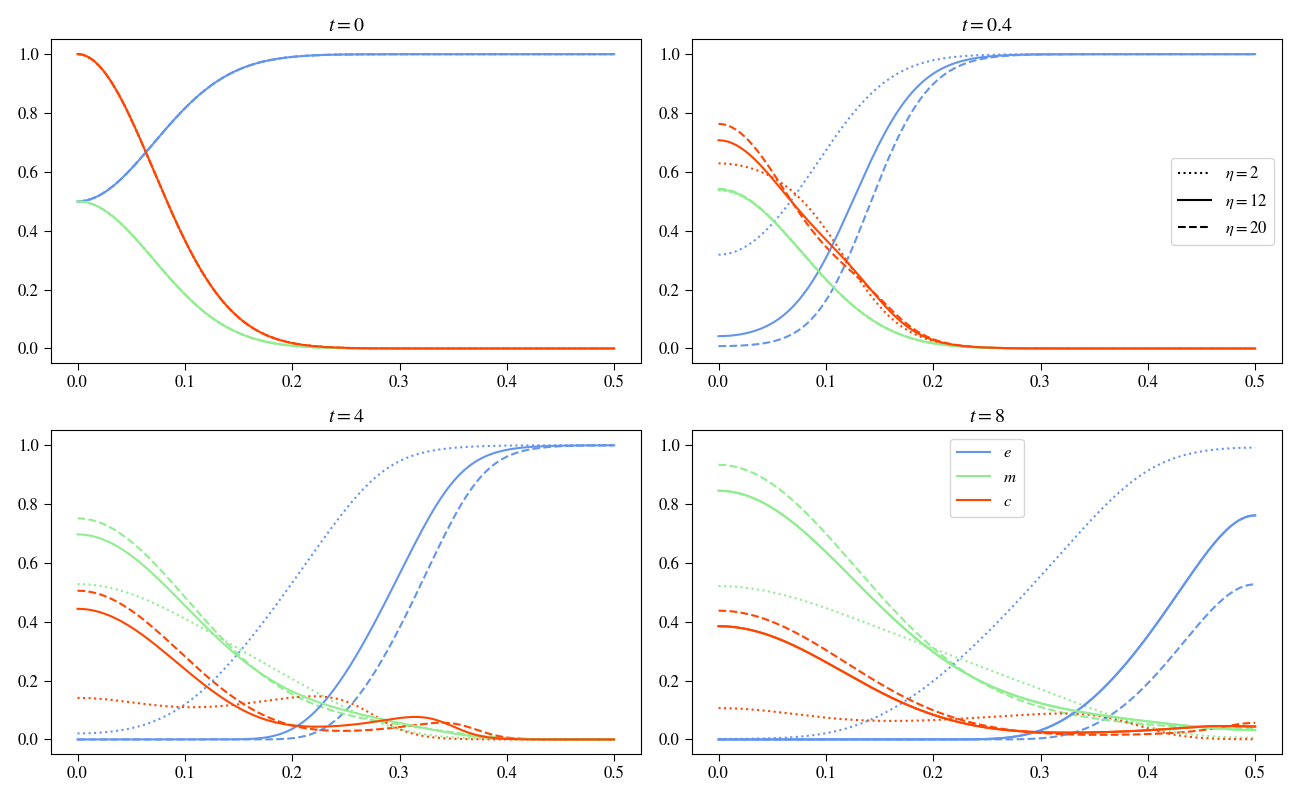
\includegraphics[width=\textwidth]{resources/images/prolif_eta_variation.png}
    \caption{Plots show results for varying $\eta$ whilst keeping the other parameters constant.}
    \label{fig:prolif_eta_variation}
\end{figure}

As we compare the $\eta$ variation between with and without proliferation and renewal models we see mostly the same effects. For the solid and dashed curves we see little though the curves of the new model are all slightly raised. Looking at $\eta=0$ we see some interesting deviations, at the time point $t=4$ the plots still look rather similar, but looking at $t=40$ we see that the curve of the tumour cells has a more even distribution along the x-axis and also its maximum is visibly lower with value of about $0.2$ at $x=1.4$ instead of $0.25$ at $x=1.3$. This behaviour is due to the renewal of the ECM, where without proliferation this curve stayed constant throughout the experiment, here it can increase, which it does altering the slope of the curve and therefore influecing the haptotatic pull for the tumour cells, additionally to this the other two experiments showed a visible increase of the tumour cell density and the matrix degrading enzyme concentration, but only a slight for the ECM concentration, here we can see no increasing of area for the tumour cell density at all. The renewal of the ECM counters the proliferation of the tumour cells and the slowed ECM degrading process in such a way that at the last two point in time we see that the ECM has visibly increased, with both curves ECM and tumour cells almost mirroring each other. Summing up the areas of both variables we see that they toghether occupy the space completely needed for the logistical growth terms, which means that proliferation and renewal will play no more important role continuing with this experiment as they have reached a equlibrium state and cancel each other out. 


\subsubsection*{$\mu_2$ Variation}
\begin{figure}[h]
    \centering
    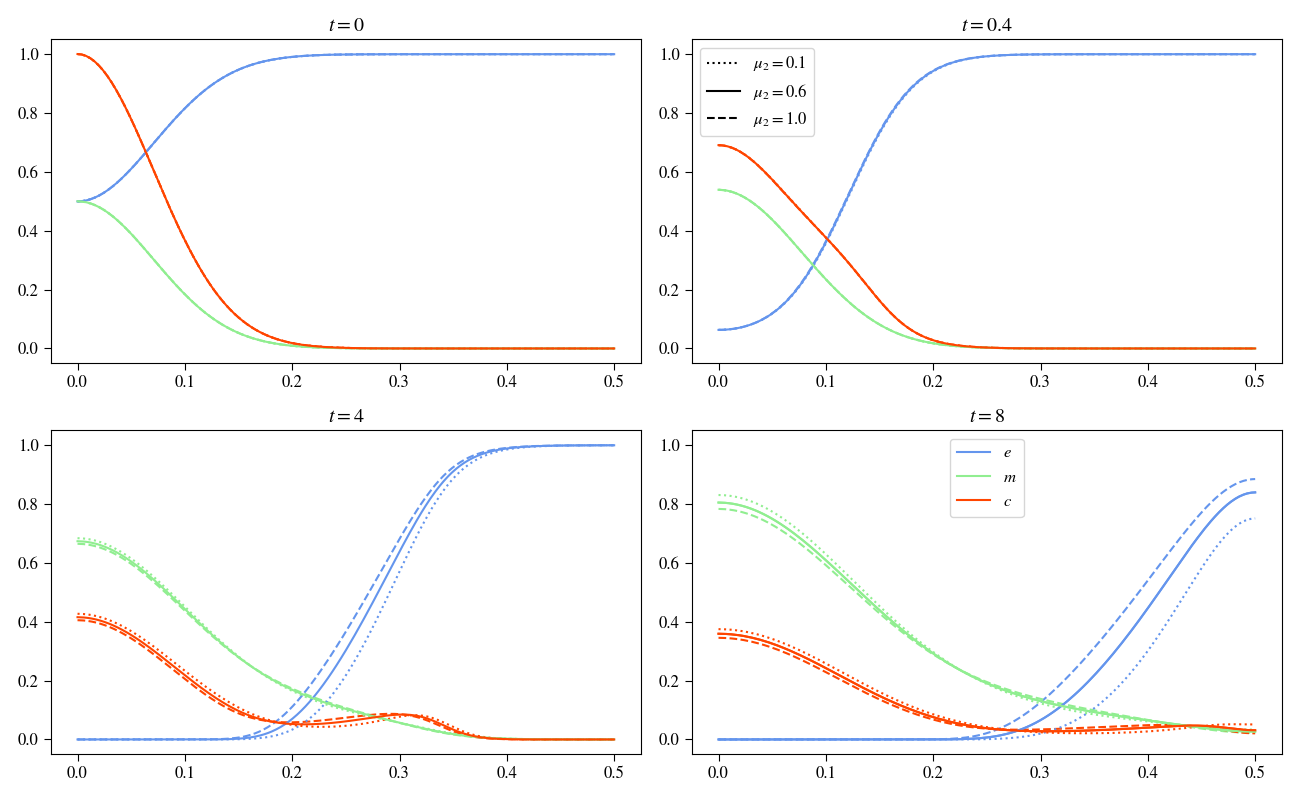
\includegraphics[width=\textwidth]{resources/images/prolif_mu_2_variation.png}
    \caption{Plots show results for varying $\mu_2$ whilst keeping the other parameters constant.}
    \label{fig:prolif_mu_2_variation}
\end{figure}

The parameter $\mu_2$ describes the renewal processes of the extra cellular matrix moleculs, with also assuming logisitcal growth in this term, being also limited by the already present ECM molecules and tumour cells.
Like we saw for $\mu_1$ the effects of $\mu_2$ need some time to show, here again we can see them after $t=40$ timesteps clearly. Wtih higher ECM renewal we see that we get slightly lower MDE maximum at $x=0$, though having stretched a little more into x-direction. The same goes for the tumour cell density, having a lower maximum at the origin, yet being more evenly distributed, whcih is due to the ECM curve being shifted slightly towards the left, intensifying the effects of haptotaxis. The last image confirms the aforementioned effects with higher ECM concentration due to renewal causes less MDE concentration at its maxima and more stretchig along x-direction, the same holding for the tumour cells. We also observe that the effects of $\mu_2$ are not as impactful on the system as the effects of $\mu_1$ were.

\subsubsection*{$d_m$ Variation}
\begin{figure}[h]
    \centering
    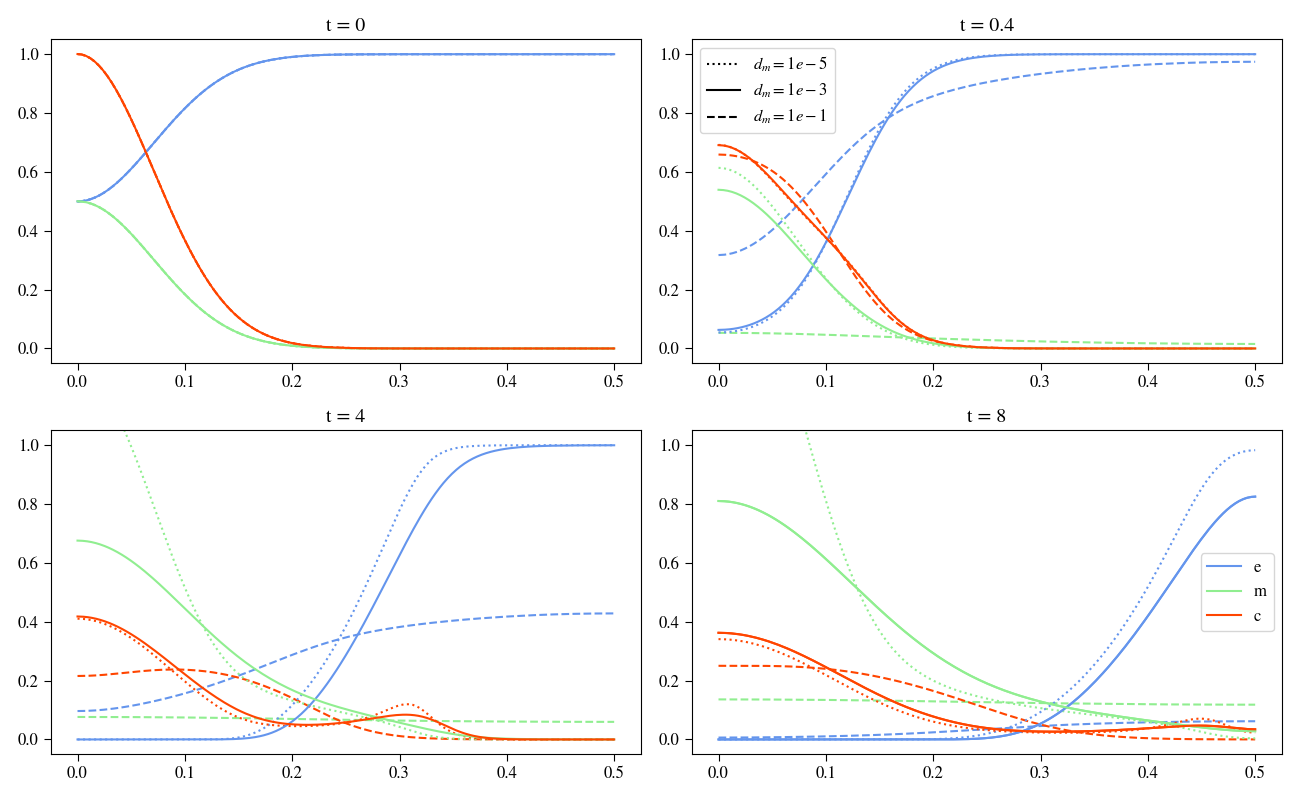
\includegraphics[width=\textwidth]{resources/images/prolif_dm_variation.png}
    \caption{Plots show results for varying $d_m$ whilst keeping the other parameters constant.}
    \label{fig:prolif_dm_variation}
\end{figure}

Comparing the results varying the diffusion factor of the matrix degrading enzymes does as before yield only minor differences between the initial and updated model. As observed before the tumour cell density's curve and the MDE concentration's curves are slightly raised due to proliferation of the tumour cells. The ECM curve for two lower values of varying $d_m$ though seem to be subject to little to no change, only for very high values of $d_m$ we can see that it is clearly raised comparing it to the model without renewal. The other two curves take off at the some point along the x-axis and finish at the same values for their ECM concentration. Looking at the tumour cell density curves for those $d_m$ values we see that towards $x=0.5$ they don't describe a as steep bump as the initial model. This causes to have little less MDE concentration as well, which is responsible for the seemingly unchanged behaviour of the extra cellular matrix concentration.

\subsubsection*{$\alpha$ Variation}
\begin{figure}[h]
    \centering
    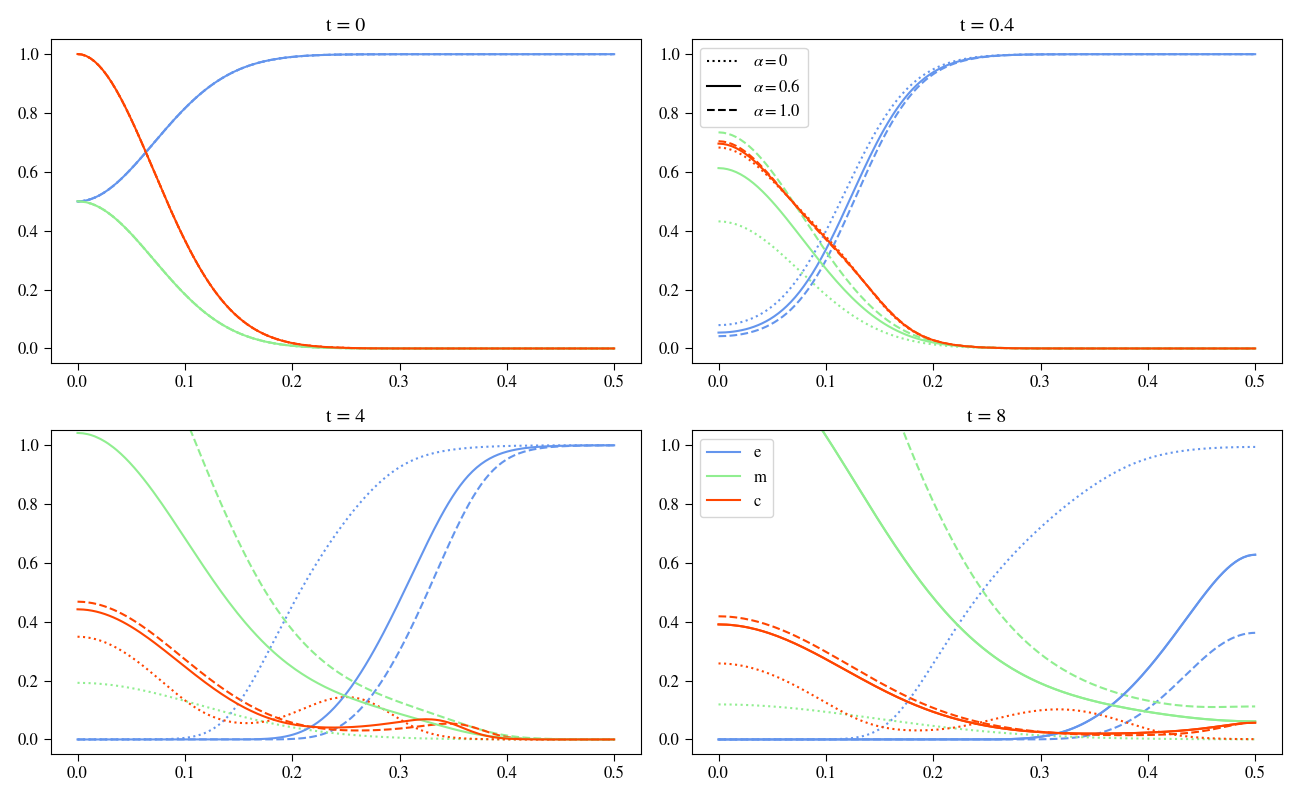
\includegraphics[width=\textwidth]{resources/images/prolif_alpha_variation.png}
    \caption{Plots show results for varying $\alpha$ whilst keeping the other parameters constant.}
    \label{fig:prolif_alpha_variation}
\end{figure}

Taking a look at comparing the $\alpha$-variation yields more interesting results since, $\mu_1$ acts as a secondary MDE production effect by producing tumour cells which in turn produce the matrix degrading enzymes. We see that though the overall shape and effects to be observed are the same, after $t=40$ the model with proliferation exceeds one at the origin for the MDE concentration for the two higher $\alpha$ experiments, where in the model without proliferation only the one with the highest $\alpha$ value did. The tumour cell denstiy curve is slightly raised, which allows the MDE concentration. Though the higher values for the MDEs leave the ECM degrading process untouched with not clearly visible difference between the inital model and the updated one. 

\subsubsection*{$\beta$ Variation}
\begin{figure}[h]
    \centering
    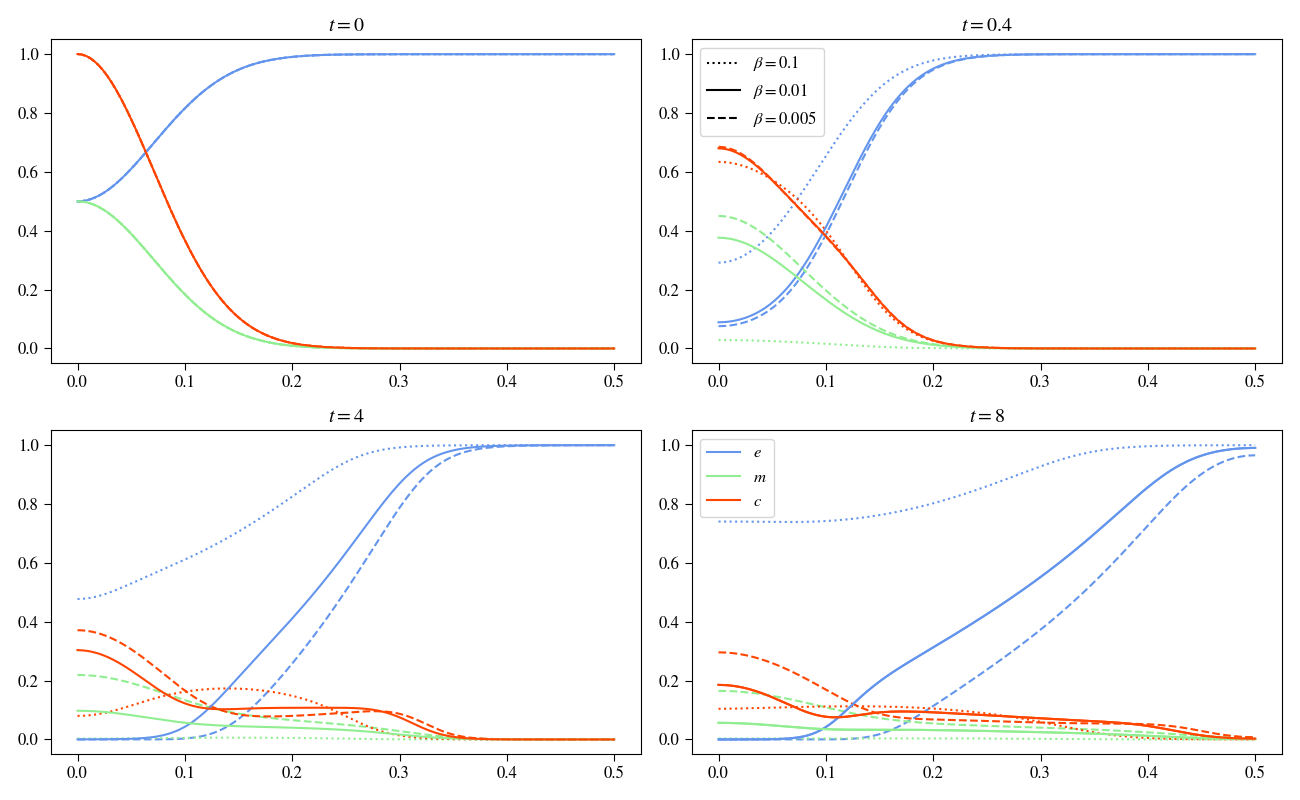
\includegraphics[width=\textwidth]{resources/images/prolif_beta_variation.png}
    \caption{Plots show results for varying $\beta$ whilst keeping the other parameters constant.}
    \label{fig:prolif_beta_variation}
\end{figure}

Considering $\beta$ we can expect that with the introduction of $\mu_2$ the ECM degradation will be slowed considerably with rising $\beta$, since this does not only reduce the MDE concentration but does also renew the ECM. Looking at the plots we can see exactly this behaviour in the dotted line, which shows the experiment results for the highest $\beta$ value of $0.1$. Though even at the end it has an overall area that is slightly less than the inital condition we can see going from timestep $t=4$ to $t=40$ that MDE decay and ECM renewal were sufficiently strong to restore the ECM and going from $t=40$ to $t=80$ we see this behaviour again, renewing the ECM. The other two experiments for $\beta$ showed no effects as strong as with $\beta=0.1$, yet we can still see the effects of proliferation and renewal especially clear in the solid line, $\beta=0.01$ at the last point in time, where we can observe a visible increase of both ECM and tumour cell density. In this experiment we see that $\beta$ is a little too low to counter the effects of ECM degradation, going from $t=40$ to $t=80$ we see a clear dicline of ECM concentration though it is not as striking as for $\beta=0.005$. 

\subsubsection*{Cross Variation}

\subsubsection*{$\mu_1 - \mu_2$ Variation}
\begin{figure}[h]
    \centering
    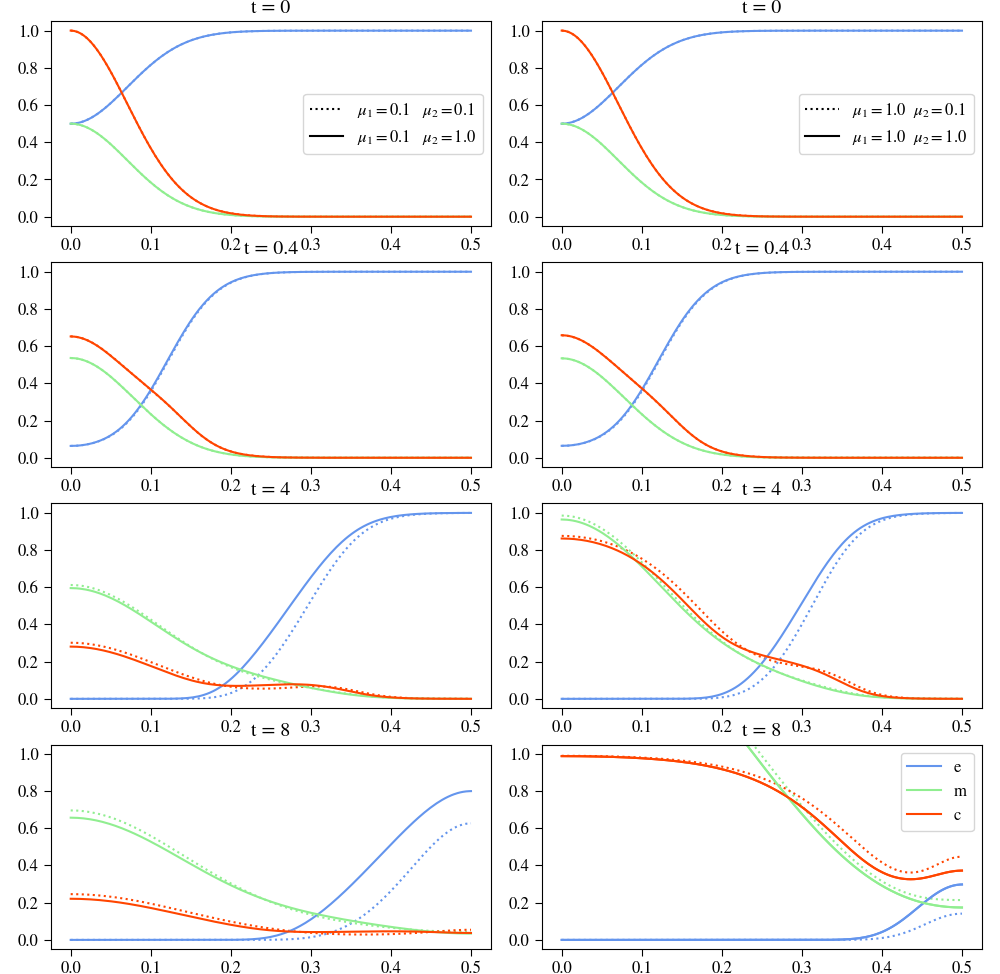
\includegraphics[width=0.85\textwidth]{resources/images/prolif_mu_1_mu_2_variation.png}
    \caption{Plots show results for varying both $\mu_1$ and $\mu_2$ whilst keeping the other parameters constant.}
    \label{fig:prolif_mu_1_mu_2_variation}
\end{figure}
The effects to observe in this cross variation take some time as did the seperate variations of both $\mu_1$ and $\mu_2$. for both $\mu_1=\mu_2=0.1$ we see that slower ECM renewal and slower tumour ell proliferation increase the degrading process of the extra cellular matrix and with this affect the haptotaxis effect to increase slightly. At the center a lump remains that has a maximum a little higher than for the experiment with $\mu_2=1.0$ and also the invasion of the tissue has proceeded a little faster. Increasing $\mu_2$, as previously mentioned, results in slower ECM degradation due to the increased renewal term and therefore the tumour cells are stretched out more evenly along the x-axis. Looking at the results when incresing $\mu_1$ we also see the effects only after $t=40$. For $\mu_2=0.1$ we see that the tumour cell density at $x=0$ is slightly larger as well as at $x\approx 2.9$ the curve for $\mu_2=0.1$ is also slightly larger being a little below $\mu_2=1.0$ in between $x\approx 0.2$ and $x\approx 0.29$. The curve for the MDEs looks very similar in both cases for $\mu_2$ due to the very similiar tumour cell density curve, c, though th eECM has visibly faster degraded for $\mu_2=0.1$ due to the slower renewal.

\subsubsection*{$d_c - \gamma - \mu_1$ Variation}
\begin{figure}[h]
    \centering
    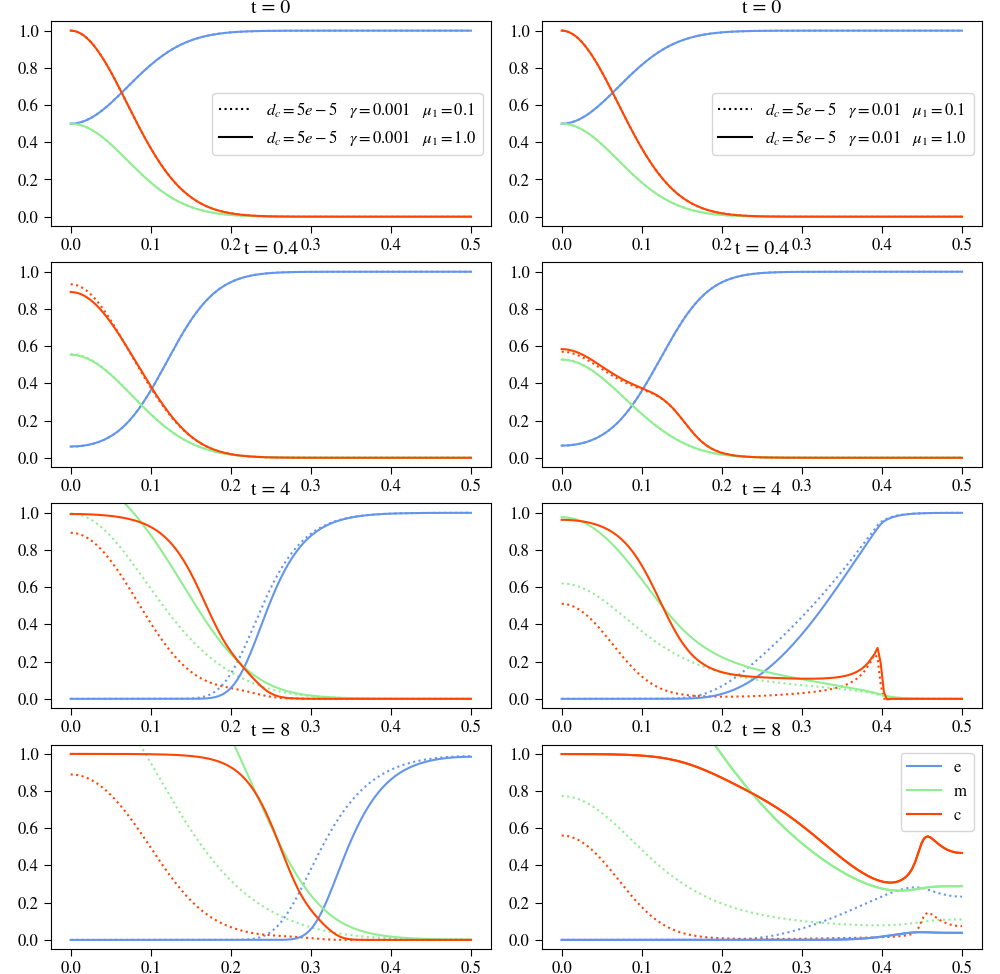
\includegraphics[width=0.85\textwidth]{resources/images/prolif_dc_gamma_mu1_1.png}
    \caption{Plots show results for varying both $d_c$, $\gamma$ and $\mu_1$ whilst keeping the other parameters constant. This plot is the first of two, with the same $d_c$ value for every plot in this figure.}
    \label{fig:prolif_dc_gamma_mu_1_variation_1}
\end{figure}

First we are goint to take a look at how chaning $\gamma$ and $\mu_1$ affects the system whils having low diffusion values for the tumour cells with $d_c=5e-5$, in figure~\ref{fig:prolif_dc_gamma_mu_1_variation_1}. Inspecting the dotted curve on the left side column, shows the results for all parameters set to low, we see that diffusion is tha mian factor for the movement of the tumour cells, with only little influence of haptotaxis, the tumour cells staying with their maximum at the center. Becasue fo this we also get a high MDE concentration there, but very little excedding the region past $x=0.3$. Due to the MDE also staying centered around thr origin the ECM there is completely degraded, though at $x=0.4$ and further still completely there. Increasing the proliferation factor to $\mu_1=1.0$ shifts the tumour cell density rightwards, making proliferation also a factor for the cell density movement, though keeping the same shape as the low proliferation factor experiment. This right shift causes the MDE concentration to also shift to the right, leading to a faster ECM degradation. Comparing these two experiments already shows the influence of proliferation.\newline
Taking now a look at the right column in figure ~\ref{fig:prolif_dc_gamma_mu_1_variation_1} we see the effects of increased $\gamma$ to $\gamma=1.0$. Foremost we see for the tumour cell density a leading edge developing, seperating it into two lumps, with one staying at the center the other invading the tissue and staying where $\nabla (c \nabla e)$ is highest. With increased $\mu_1$ this secession moving into the tissue is getting more pointy, defying differentiability. After $t=40$ we can ovserve clear differences regarding ECM and MDE concentration. We see that for higher $\mu_1$ we also get a higher MDE concentration which degrades the ECM visibly faster at the end of the experiments at $t=80$. Though interestingly at $t=40$ the ECM degradataion difference is only minor, at the last point in time the accellerated tumour cell proliferation shows its effet with producignmore MDEs and degrading the ECM considerably faster. What is also interesting to note is that increasing $\gamma$ and keeping $\mu_1$ low the total area of the MDE concentration is lowered also.
Increasing now $d_c$ to $0.1$ we see for all experiments in figure~\ref{fig:prolif_dc_gamma_mu_1_variation_2} that the diffusion of the tumour cells was sufficiently high to evenly distribute the tumour cells constatnly in the space. This constant distribution allows to get an even better look at how $\mu_1$ affects the results, by seeing the lines, describing the tumour cells, rise through time. Looking at the tumour cells over time we can see no observable difference for varying $\gamma$. Haptotaxis effects are completely overlaid by diffusion. We see in the left column that if keeping dc high and $\gamma$ low, but increasing $\mu_1$ leads to higher MDE production rates and also faster ECM degradation. The same behaviour is observable in the right column showing the results for high $\gamma$. That we see no difference is clear, since the tumour cell density development is identical over time as mentioned above. 

\begin{figure}[h]
    \centering
    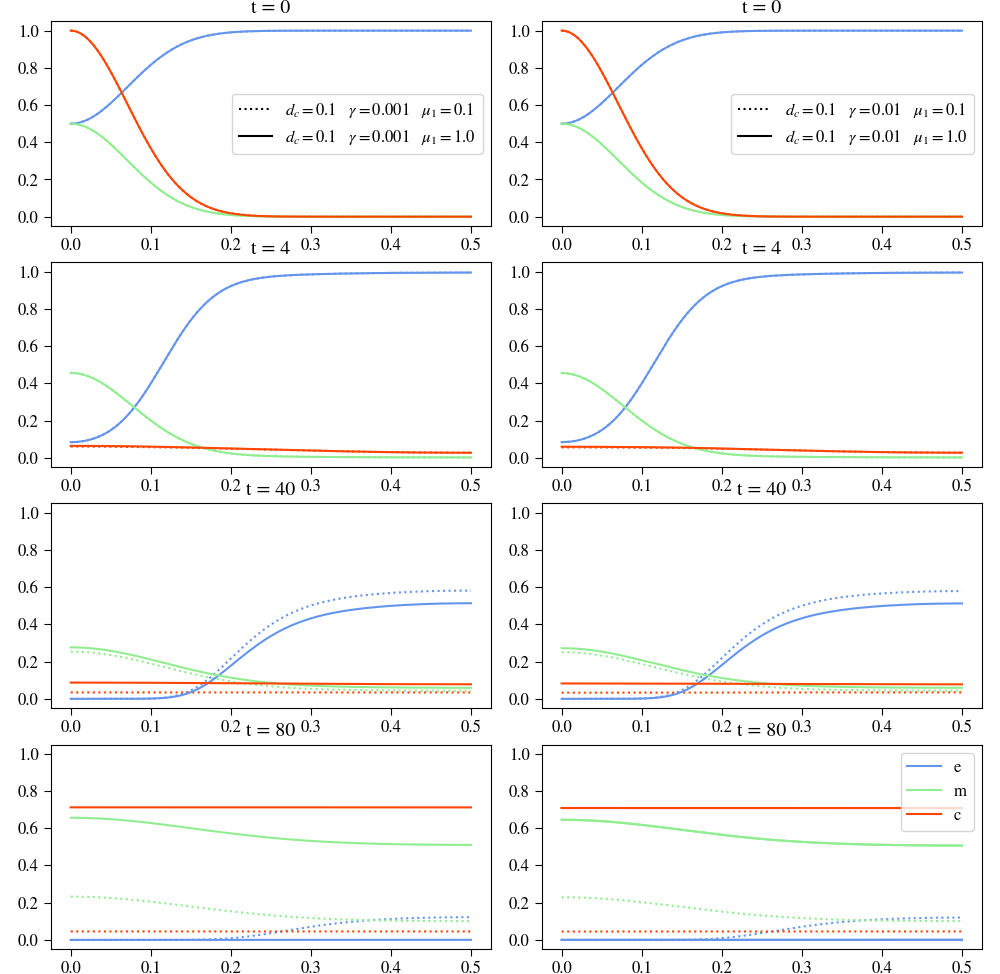
\includegraphics[width=0.85\textwidth]{resources/images/prolif_dc_gamma_mu1_2.png}
    \caption{Plots show results for varying both $d_c$, $\gamma$ and $\mu_1$ whilst keeping the other parameters constant. This plot is the second of two, with the same $d_c$ value for every plot in this figure.}
    \label{fig:prolif_dc_gamma_mu_1_variation_2}
\end{figure}

\subsubsection*{$\eta -\mu_2$ Variation}
\begin{figure}[h]
    \centering
    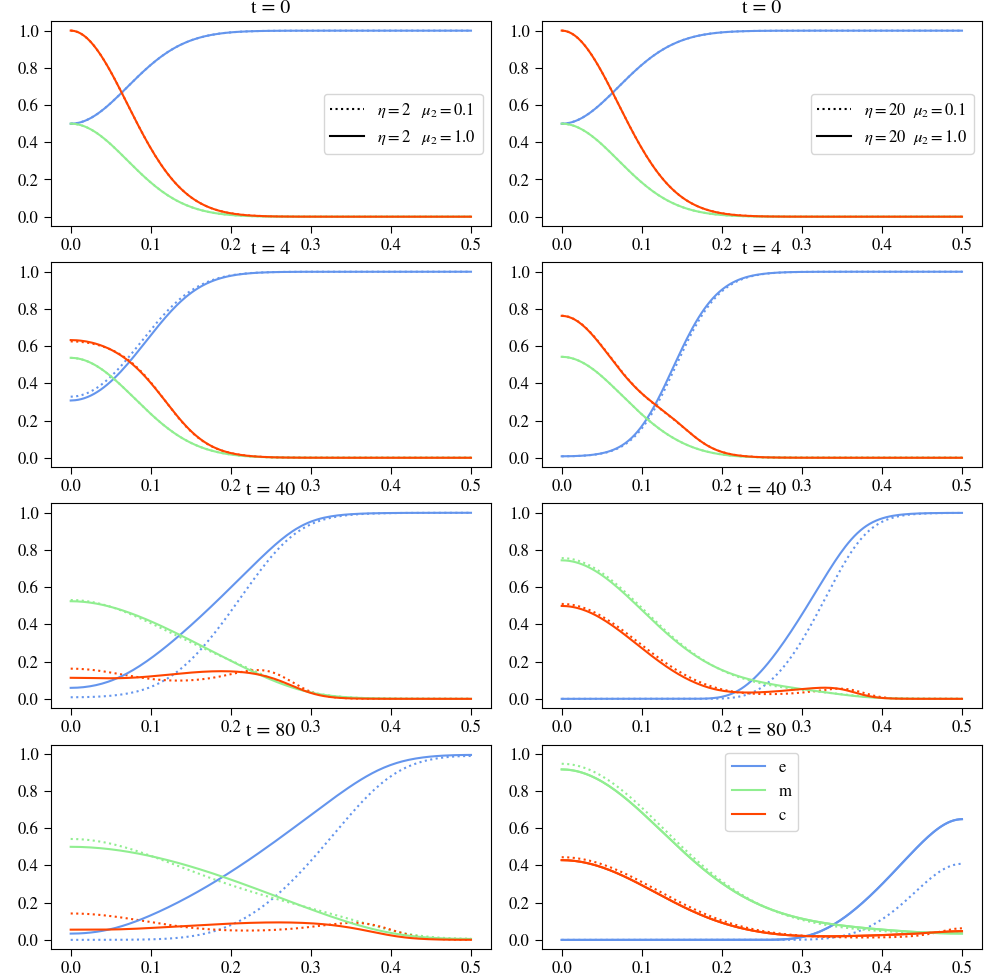
\includegraphics[width=0.85\textwidth]{resources/images/prolif_eta_mu2_variation.png}
    \caption{Plots show results for varying both $\eta$ and $\mu_2$ whilst keeping the other parameters constant.}
    \label{fig:prolif_eta_mu_2_variation}
\end{figure}

Varying both $\eta$ and $\mu_2$ we can expect to see clear changes in the curve describing the ECM concentration. On the left side of figuer~\ref{fig:prolif_eta_mu_2_variation} we can see the two experiments for low $\eta$ values and see that increasing $\mu_1$ has only a little effect. Where we could have expected to maybe even see an increase of the ECM we see that the ECM curves for both experiments verify that the renewal factor $\mu_2$ was too low to counter the ECM degradation, even with a low degradation factor. Still between $\mu_2=0.1$ and $\mu_2=1.0$ there are visibe differences in the degrading speed of the ECM. We can also observe that with the higher renewal term the tumour cell density curve receives more of an effect of haptotaxis resulting in an more streteched curve with only one long lump of tumour cells, where for the lower renewal factor we can still clearly see that there is a secession that invades the tissue and one that stays at the origin. Concerning the MDE curves we can see little difference, for higher $\mu_2$, which meant more stretched tumour cell density, we can also observe a more stretched MDE curve with a lower maximum at the origin. \newline 
Taking now a look at the experiments with raised $\eta$ to accellerate the ECM degrading process, we can only see pregnant differences in the curve describing the ECM concentration, the other two look across the steps in time to be widely similar. For the ECM curve we see that the experiment with the lower $\mu_2$ value results in a faster degradation process.




\subsection{Three Dimensional Results}
\subsubsection{Replicating Results}
\subsubsection{Parameter Analysis}
\subsection{Three Dimensional Simulations with Heterogenous ECM Structure}
